% !TEX root = ../thesis_main.tex
% 
% 
% 
% 
%%%% --- * --- %%%%	
\chapter{Simulations}
\label{simulations_chapter}
%I really need an excuse to include more pictures of data.  Also, more pictures of simulations.
\missingfigure{Show simulated spectra separated by scattering category.}
\missingfigure{Show SimpleMC spectra, show the supersum, show the superratio, show the superratio asymmetry.  Maybe do some simple fits to show how much better the superratio asymmetry is than \emph{not} the superratio asymmetry.  }

%\note[color=done]{John says:  ``I doubt I will have further useful comments on the Ch. ((this chapter)) as they are now.'' -- Yeah, but *now* he will.}

The TRINAT collaboration has created a Geant4 (G4) simulation which models the geometry and materials within the experimental chamber, and uses a monte carlo algorithm to describe generalized physical processes such as particle scattering and energy loss, within the geometry specific to the experiment.  This software library has been maintained and updated over several generations of graduate students~\cite{ben_thesis}~\cite{spencer_thesis}.  
\note{add comment about how  you need G4 to do scattering/backscattering.  I think I wrote a blurb like this *somewhere* already....}

\section{Considerations for Software Upgrade Implementation}
\label{sec:software_upgrades}
Prior to the simulations required for this particular experiment, two different sets of changes to the G4 code were needed -- the first to enable multithreading, and the second to introduce certain BSM interactions to the decay distribution.  

Enabling multithreading allows for a single instance of the Geant4 simulation to run on several processors at once, effectively speeding up the overall simulation by a factor of the number of processors used.  In the years since the simulation was originally created, the Geant4 collaboration had created libraries intended specifically to support multithread usage, and since the running G4 simulations had historically been very time consuming for the TRINAT collaboration, the decision was made to implement multithreading within our own monte carlo software, on the hopes that this would enable faster progress in analysis. 

Enabling multithreading support turned out to be quite time consuming, and in the end it might have been faster to have spent those months running simulations one processor at a time.  Perhaps the improvement will prove valuable for use in future TRINAT experiments.  

%Throughout the history of this simulation package, 
The TRINAT G4 monte carlo package had never been used to directly model interactions beyond the standard model within the decay physics.  
\aside{because for $\Abeta$ even a BSM interaction will *basically* look like a SM interaction, and I think something somewhere isn't precise enough to distinguish it.}  
It had  previously been set up by the collaboration to use a probability density function (PDF) including most of the terms from Holstein's Eq. (51)~\cite{holstein}, which describes both electron and neutrino momenta from polarized beta decay.  This treatment is quite robust, and includes corrections at recoil-order, as well as certain other corrections of similar size.~\aside[color=bluetodo]{which other corrections?  coulomb and/or radiative corrections, but somehow when I say that, I'm apparently talking about a different thing than everyone else who uses those terms.  also, weak magnetism. also ... ???}

Unfortunately, terms arising from interactions beyond the standard model are not included in Holstein's description of the decay process. \aside{Is this true?  Does it not include *any* BSM interactions?}  To understand the kinematic results of the exotic interactions of interest to us here, we turn to the classic JTW treatment of beta decay~\cite{jtw}~\cite{jtw_coulomb}.  In addition to the (expected) vector and axial interactions, JTW also describes the interaction in terms of (exotic) scalar and tensor interactions, should such be present.  
\note{Furthermore, although it is currently understood that the weak interaction is predominantly or perhaps entirely `left-handed', the JTW treatment leaves certain phase angles unfixed, and is therefore able to accurately describe a decay which is, for example, partially `right-handed' -- however the latter feature is not directly relevant to the project at hand.  [It's several phase angles in JTW, but maybe it's fundamentally only like one angle on some level?  Also I think it's not actually a ``gauge freedom,'' per se.  .... No, I'm pretty sure this `phase angle' description is all wrong.]  Also, consider time reversal!  Anyway, most of this paragraph probably goes better in Section~\ref{sec:math_formalism}.}
Despite JTW's broad ability to describe beta decay under a variety of physical models, this treatment includes only the leading-order terms, and smaller terms, such as recoil-order corrections, are neglected entirely.  

\note[color=org]{Surely I describe what recoil-order corrections even *are* in some appendix somewhere, right?  Or, possibly, in Section~\ref{sec:math_formalism}.  Possibly the paragraphs above need to be moved...}

Because the present project is a precision measurement of the Fierz interference, a term which arises from scalar and tensor couplings, it was imperative to create an event generator for our G4 simulations that could account for these exotic interactions while also including in its PDF the higher-order effects which, in some cases, can mimic the effects of a scalar or tensor current.  

While it might have been possible to directly combine JTW's result with Holstein's Eq. (51), it should be noted that JTW's expression is not compatible in general with the principle of conservation of momentum;  as recoil momentum is neglected entirely, the description is only of two leptons emerging from a nucleus in directions that do not directly oppose one another.  Therefore, the prospect of combining these two slightly incompatible expressions directly might be enough to give one pause.  On an experimental level, the mathematical description of an emerging neutrino is only of interest to us to the extent we can reconstruct it based on detecting both a beta and the recoiling nucleus from a single decay event, and within the present experiment we do not have simultaneous access to both a beta detector and a recoil detector.  

In light of the above considerations, it was decided that an entirely new event generator must be created, based instead on Holstein's Eq.~(52), in which neutrino momentum has been integrated over and is therefore no longer an explicit part of the PDF~\cite{holstein}.  As one might guess, Holstein's Eq.~(52) is greatly simplified in comparison to Holstein's Eq.~(51).  A similar integration over all possible neutrino momenta can also be performed on the JTW PDF, causing several terms to vanish.  The result in both the Holstein and JTW cases is a PDF over only beta energy and direction as measured with respect to nuclear polarization, and the two expressions can be combined in a straightforward manner by comparing similar terms.  

It is this combined Holstein+JTW expression that forms the basis of the new G4 event generator.  It must be noted that although the largest effect from any present scalar or tensor interactions would likely (depending on certain phase angles) be in a non-zero value of $\bFierz$, these interactions can also introduce a perturbation to $\Abeta$ at a higher order.  In order for any precision experimental measurement of $\bFierz$ to be generalized to limits on the parameter space of scalar and tensor currents, it is important to incorporate an accurate representation of the results of such exotic interactions on \emph{all} available observables, and the new G4 event generator does this.  

\note{Things that the G4 simulation did that I kept include:  an accurate representation of the complex details of our experimental geometry.  Also, the noise spectra on the DSSDs.}


\FloatBarrier
\section{The Simple Monte Carlo and Response Function}
\label{sec:responsefunction}
Scattering (both forward scattering and backscattering) is an important effect to consider within this experiment, and it must be evaluated through extensive and time consuming monte carlo simulations -- in this case, using Geant4.  However, there are a number of other systematic uncertainties that must also be evaluated, and it is computationally prohibitive (even after multithreading support was implemented) to evaluate all of them via the same sort of high statistics, scattering included, full monte carlo that we use for scattering effects.  Luckily, the systematic effects arising from scattering are largely decoupled from other effects, and this section describes the framework that has been implemented in order to evaluate certain other systematic effects separately.  

%However, while scattering effects are a dominant source of systematic error, \aside[color=org]{It's *the* dominant error, right?  Right?  Also, maybe point at that final error budget table here.} other systematics cannot simply be neglected.  
%Because of the large number of systematic effects to be examined, and because of the processor time required to run a high statistics Geant4 simulation even after enabling multithreading support, it was desirable to develop a procedure by which it would be possible to evaluate certain systematic effects while avoiding the computationally intensive simulations that might traditionally be used.  

To this end, a fast-running Simple Monte Carlo (SMC) was developed together with an empirical ``response function'' similar to the one described by Clifford et al~\cite{clifford} to describe probabilistic beta energy loss before its detection in a scintillator.  In the end, the lineshape description became quite involved, and it is unclear whether, in the end, any time was saved this way. 

The purpose of the SMC was to \emph{quickly} generate initial particle kinematics probabilistically for beta decay events, and it uses the very same event generator based on Holstein's Eq.~(52)~\cite{holstein} that was developed for use with the more sophisticated Geant4 simulations.~\aside{Reference previous section where I discuss this, maybe?}  However, unlike in a G4 simulation, the SMC makes no attempt to track particles through the chamber, and instead simply calculates detector hits based on initial particle momentum.  This procedure obviously neglects scattering effects, which can (in differing regimes) both \emph{increase} and \emph{decrease} the number of beta particles incident on a detector.  Furthermore, this procedure also neglects any energy absorption in materials through which the beta passes before hitting a scintillator -- and the beta \emph{must} pass through several such materials (see Fig.~\ref{chamber_decayevent}).

To make the best use of the SMC for evaluating systematic errors, the energy lost before a beta hits a scintillator must be accounted for somehow in order to ensure all relevant physical effects are propagated through.  In particular, before hitting a scintillator, a beta must pass through a $275\,\mu m$ thick silicon carbide mirror, a $229\,\mu m$ thick beryllium foil, %used to separate the inner portion of the vacuum chamber from the outside world
and finally a set of $300\,\mu m$ thick double-sided silicon strip detectors (DSSDs), before finally having its remaining energy absorbed within a scintillator.  Although the DSSDs are themselves detectors with the ability to record the amount of energy deposited by an incident particle, there are some known problems in achieving a uniform level of precision across the full surface of the DSSDs,\aside{See:  Some other section?  Maybe?} so adding the DSSD energy back to the scintillator energy to produce a better estimate of the original beta energy has the potential to create some problems for the analysis.  Furthermore, given the presence of the mirror, an object with a similar thickness and scattering properties to the DSSDs, re-adding the energy lost in the DSSDs would not eliminate the need to estimate probabilistic energy loss in similar materials.  

In order to create a quantitative description of the effective response function, which varies with initial beta energy, an analytic function of 14 parameters \aside{Is it definitely 14 of them?} has been created to model scintillator output for decays from the central cloud for each of the two polarization states in use.  In other words, although the form of the model is always the same, the 14 individual parameters will take different values for each of the four detector and polarization combinations.  The full response function model is given by the expression,
%for each of four detector and polarization combinations (56 parameters in total), to represent the final beta energy spectra in the scintillators.  
\bea
	R(E_{0}, \textrm{Detector}, \mathrm{Polarization}) &=& p_{\textrm{norm}} \left( f_{\mathrm{moyal}} + f_1 + f_2 + f_3 + f_4 + f_5 \right) + f_{511},
	\nonumber \\
	\label{eq:fullresponsefunction}
\eea
where $p_{\textrm{norm}}$ is one parameter, and the other terms within the expression are themselves functions of multiple parameters and are given by,

% !TEX root = ../thesis_main.tex
%
%
%
%%%% --- * --- %%%%	
%\bea
\begin{flalign}
f_{\mathrm{moyal}} \,\, = \,\, & 
	(1-p_{\mathrm{gfrac}}) \left( 1 + \frac{-p_\alpha - p_\beta }{\left| E_0 \right|} - \frac{p_\Delta}{ p_\gamma \, p_{W} } - p_\gamma \, p_{W} \right)  
	 && \nonumber \\ 
	 & \,\:\;\;\:\, \,\:\;\;\:\, \,\:\;\;\:\, \,\:\;\;\:\, \,\:\;\;\:\, \,\:\;\;\:\,
	 \times \left( 
	\frac{ e^{ \left( \frac{ x-\left( E_0-\frac{1}{2}p_{\mathrm{dE0}} \right) }{ 2 \, p_{\mathrm{lres}}\left|E_0-\frac{1}{2}p_{\mathrm{dE0}}\right| } \right) }  e^{\left(-\frac{1}{2} e^{\left( \frac{x - \left(E_0-\frac{1}{2}p_{\mathrm{dE0}} \right) }{ p_{\mathrm{lres}} \left| E_0-\frac{1}{2}p_{\mathrm{dE0}} \right| } \right)} \right)} }{\sqrt{2\pi \, p_{\mathrm{lres}} \left| E_0-\frac{1}{2}p_{\mathrm{dE0}} \right| } } 
	\right), &&
	\label{eq:fmoyal}
\end{flalign}
%\eea

\note{Obviously, from a physical standpoint, the initial beta energy $E_0$ must be positive, but the response function still includes several expressions of the form, $\left| E_0 \right|$.  This is not done by accident, but rather is an intentional adjustment used to encourage the parameters to behave well within a fit. }
% !TEX root = ../thesis_main.tex
%
%
%
%%%% --- * --- %%%%	
\begin{flalign}
	f_1() \,\, = \,\, & p_{\mathrm{gfrac}}  \left( 1 + \frac{-p_\alpha - p_\beta }{\left|E_0\right|} - \frac{p_\Delta}{ p_\gamma \, p_{W} } - p_\gamma \, p_{W} \right) \!
	\left( 
	\frac{ e^{\left( - \frac{ \left(x-\left(E_0+\frac{1}{2}p_{\mathrm{dE0}}\right) \right)^2 }{ 2 \, p_{\textrm{toeres}} \left| E_0+\frac{1}{2}p_{\mathrm{dE0}} \right| } \right)} } { \sqrt{2\pi \, p_{\textrm{toeres}} \left|E_0+\frac{1}{2} p_{\mathrm{dE0}}\right|} }
	\right), &&
	\label{eq:f1}
\end{flalign}
\begin{flalign}
	f_2() \,\, = \,\, & \frac{p_\alpha}{\left|E_0\right|} \left( \frac{1 - \Erf\left[ \frac{(x-\left|E_0\right|)}{\sqrt{2 \, p_{\textrm{toeres}} \left| E_0 \right| }} \right]}{2 \, \left| E_0\right| } \right),
	&&
	\label{eq:f2}
\end{flalign}

\note[color=bluetodo]{In these response functions, $x=$?}
% !TEX root = ../thesis_main.tex
%
%
%
%%%% --- * --- %%%%	
\begin{flalign}
	f_3 \,\, = \,\, & \frac{p_\beta}{\left|E_0\right|}  \left( 	\frac{ e^{ \frac{ p_{\mathrm{k}} *(x-E_0) }{ \left|E_0\right|} } * e^{ \frac{p_{\textrm{toeres}} \, p_{\mathrm{k}}^2 }{2 \left|E_0\right|} } }{ 2 (1-e^{-p_{\mathrm{k}}} ) } \right)
	\left(1 - \Erf\left[ \frac{ (x-E_0+p_{\textrm{toeres}} \, p_{\mathrm{k}} ) } {\sqrt{2 \,p_{\textrm{toeres}} \left|E_0\right| } } \right] \right), &&
	\label{eq:f3}
\end{flalign}
\begin{flalign}
	f_4 \,\, = \,\, & \frac{p_\gamma}{2}   \left( \Erf \left[ \frac{ x-E_0 }{ \sqrt{(2 \, p_{\textrm{toeres}} \left|E_0\right| )} }  \right]  
	- \Erf \left[ \frac{ x-E_0-p_{W} }{ \sqrt{2 \, p_{\textrm{toeres}} \left| E_0+p_{W}\right| } } \right] \right), && 
	\label{eq:f4}
\end{flalign}

\note{To evaluate $\Erf\left[\right]$ for parameter fits, root's built-in function was used.  Root also includes a built-in Landau function, but it makes everything very slow if we use it.}
% !TEX root = ../thesis_main.tex
%
%
%
%%%% --- * --- %%%%	
\bea
	\!\! f_5 \, &\!\!= \,\,& \!\! \frac{p_{\Delta}}{2 \, p_{\gamma} \, p_{W}^3 }  
	\left[  
	(E_{\textrm{out}}-E_{\textrm{in}}) \left( \Erf\left[ \frac{(E_{\textrm{out}}-E_{\textrm{in}}) }{ \sqrt{2 \, p_{\textrm{toeres}} \left|E_{\textrm{in}}\right| } } \right] 
	- 2 \, \Erf\left[ \frac{ (E_{\textrm{out}}-E_{\textrm{in}}-p_{W}) }{ \sqrt{2 \, p_{\textrm{toeres}} \, \left| E_{\textrm{in}}+p_{W}\right| }} \right]
	\right. 
	\phantom{\left( \frac{e^{\left(\frac{(p_{W})^2}{ \left| E_{\textrm{in}} \right|} \right)}}{\sqrt{2 \left|E_{\textrm{in}} \right| }} \right) \!\!\!\!\!\!\!\! \!\!\!\!\!\!\!\! \!\!\!\!\!\!\!\! \!\!\!\! \!\!} %% phantom to get to get bracket size right..
	\right. \nonumber \\ && \left. \left.
	%
	+ \Erf\left[ \frac{(E_{\textrm{out}} - E_{\textrm{in}} - 2 p_{W}) }{ \sqrt{2 \, p_{\textrm{toeres}} \, \left| E_{\textrm{in}} + 2 p_{W}\right| }} \right] \right) 
	+ (2 \, p_{W}) \left( \Erf\left[ \frac{(E_{\textrm{out}}-E_{\textrm{in}}-p_{W})}{\sqrt{2 \, p_{\textrm{toeres}} \left|E_{\textrm{in}}+p_{W}\right| }}\right] 
	\right. \right. \nonumber \\ && \left. \left.
	%
	- \Erf \left[ \frac{(E_{\textrm{out}}-E_{\textrm{in}} - 2 p_{W})}{\sqrt{2 \, p_{\textrm{toeres}} \left| E_{\textrm{in}}+2 p_{W}\right| }} \right] \right) 
	+ \left( 2\, p_{\textrm{toeres}} \left| E_{\textrm{in}} \right| \right)  \left( \left( \frac{e^{\left(\frac{- (E_{\textrm{out}}-E_{\textrm{in}})^2}{(4\,p_{\textrm{toeres}} \left| E_{\textrm{in}}\right| )} \right)} }{\sqrt{2 \pi \, p_{\textrm{toeres}} \left| E_{\textrm{in}} \right| }}\right) 
	\right. \right. \nonumber \\ && \left. \left.
	%
	+ \left( \frac{ - 2 e^{ \left(\frac{ - (E_{\textrm{out}}-E_{\textrm{in}}-p_{W})^2 }{(4 \, p_{\textrm{toeres}} \, \left| E_{\textrm{in}}+p_{W}\right| )} \right) } }{( \sqrt{2\pi \, p_{\textrm{toeres}}\left| E_{\textrm{in}}+p_{W}\right| } )} \right) 
	+ \left( \frac{e^{\left(\frac{ - (E_{\textrm{out}}-E_{\textrm{in}} - 2 p_{W})^2}{(4 \, p_{\textrm{toeres}} \, \left| E_{\textrm{in}} + 2 \, p_{W}\right| )} \right)}}{\sqrt{2 \pi \, p_{\textrm{toeres}} \left|E_{\textrm{in}} + 2 \,p_{W}\right| }} \right) 
	\right) \right],
%	\!\!\!\!\!\!\!
%	\nonumber \\
	\label{eq:f5}
\eea
 and
% !TEX root = ../thesis_main.tex
%
%
%
%%%% --- * --- %%%%	
\bea
	f_{511} &=& 
	\left| p_{\mathrm{scale}} \right|
	\left[ \left( \frac{195}{17} \sqrt{\frac{2}{\pi}} \, e^{\left(\frac{-(E_{\textrm{in}} - 308)^2}{578}\right) } \right)  
	+ \left(40 + \frac{(E_{\textrm{in}} - 210)^2}{900} \right) \! \left( 1 - \Erf\left[\frac{E_{\textrm{in}} - 334}{30}\right] \right) \!\!\!\! 
	\right. \nonumber \\ && \left.	
	+ \left( \frac{ (E_{\textrm{in}} -505)^2 }{1440}\right) \! \left( 1 - \Erf\left[ \frac{E_{\textrm{in}} - 505}{30}\right] \right) \! \left(1 + \Erf\left[\frac{E_{\textrm{in}}-334}{30}\right] \right)  
	\phantom{e^{\left(\frac{(E_{\textrm{in}})^2}{5} \right)  }} 
	\!\!\!\!\! \!\!\!\!\! \!\!\!\!\! \!\!\!
	\right],
	\label{eq:f511}
\eeawhere a $p$ with any subscript is taken to be a variable parameter that must be evaluated.  The expressions $f_1$, $f_2$, $f_3$, $f_4$, and $f_5$ are motivated by or taken directly from expressions of the same name within Clifford's description, and the individual parameters $p_\alpha$, $p_\beta$, $p_\gamma$, $p_\Delta$, $p_W$, and $p_k$ are closely related to their counterparts of similar name~\cite{clifford}.  The expressions $f_{\mathrm{moyal}}$ and $f_{511}$ represent a departure from the published treatment, however, and arise from physical behaviours within this experiment which are not described within Clifford's treatment.

In particular, $f_{511}$ is a rather inelegant representation of the annihilation radiation compton edge within our geometry.  Although the DSSD provides an effective veto for the overwhelming majority of these events--and indeed within Clifford's treatment this veto is treated as being perfect in its discernment--it is clear both from experimental spectra and the Geant4 simulations intended to represent them that there exist a small number of such events within our scintillator spectra that cannot be vetoed in this manner.  These events must be understood and adequately accounted for.  

It should be noted that no attempt is made to derive the expression for $f_{511}$ from first principles; the expression was chosen only because of its visual similarity to the spectrum's fit residuals before its inclusion.  This expression's contribution to the overall function is negligible at all but the lowest initial beta energies (Eq.~\ref{eq:f511}'s $p_{\mathrm{scale}}$ parameter, showing the absolute normalization of $f_{511}$, is plotted in the top right of Fig.~\ref{fig:lineshapeparams_scale}.), and is always negligible at scintillator energies above $\sim 500\,$keV, as can be seen in Fig.~\ref{fig:lineshape_750}.  We note that within the final analysis, all scintillator spectra will be given a low energy cutoff at 400\,keV, so the only the higher energy tail of $f_{511}$ will make any contribution.  \aside{Also, I think for this particular part of analysis, the cutoff was like 600 keV.} \aside[color=org]{Some of this content needs to go somewhere else.}

The expression $f_{\mathrm{moyal}}$ arises from the beta particles' energy loss within materials (i.e. the mirror, the beryllium foil, and the DSSD itself, as in Fig.~\ref{fig:thechamber}) before its eventual absorption within the scintillator.  Although Clifford's treatment does include a $\Delta E$ detector (our DSSD would be the equivalent), the energy absorbed in this detector is added back in to the total before Clifford's final spectra are modeled.  Although it would be possible to do something similar with our DSSD spectra, \aside[color=org]{We never attempt to do this, because reasons.  Don't I talk about this somewhere?} we would still be left with the problem of accounting for the similarly-shaped energy loss within the mirror and foil. 

The distribution for energy deposition within a thin material by an energetic charged particle, first described by Lev Landau in 1944~\cite{landaudistribution}, is now known as a Landau distribution.  This distribution has a variety of properties that make it challenging to work with -- notably its mean, variance, and all higher moments are undefined, and the distribution itself cannot be written in closed form.  Its primary redeeming mathematical feature, however, is the fact that the convolution of a Landau distribution with another Landau distribution is, itself, a Landau distribution, and this means that we can represent the sum total of energy absorption within three successive thin materials as a single Landau distribution.  

Within the present context, an expression for energy absorption that can be evaluated and re-evaluated quickly by computer with adjusted parameters is needed, as this must be used within a fit function.  To this end, we employ a so-called `Moyal function', which was developed in 1955 to be used as a closed form approximation to the Landau distribution~\cite{moyal}.  Indeed, Eq.~\ref{eq:fmoyal} is little more than a Moyal function.  
\note{...as previously mentioned, re-introducing the energy from the BB1s invites problems with maintaining a uniform energy threshold over the entire detector. }
\note{somewhere I have to talk about the empirical noise spectrum etc. on the BB1s.  Or maybe I've already mentioned it somewhere.}  

The values of these parameters are allowed to vary with initial beta energy, and must be determined empirically by a series of fits to simulated spectra.  
%Since the final response function is expected to be a function of initial beta energy, we must allow for these parameters to also vary as a function of initial beta energy.  
To effect this result, the TRINAT Geant4 simulation is used to generate a series of `mono-energetic' spectra.  That is, for each energy value under consideration (with discrete values selected to span the energy range of betas in our decay), events are generated in which every outgoing beta initially has the same amount of kinetic energy, and the angular distribution of these betas is physically appropriate for the polarization and beta energy under consideration.  These mono-energetic betas are propagated through the experimental geometry via Geant4, and the resulting scintillator spectra are recorded.  Each polarization state must be considered separately, but spectra for both detectors are generated simultaneously, as it is necessary to generate events into a full $4\pi$ steradians in order to fully account for betas scattered into- or away from the detectors.  Cuts identical to those imposed on the experimental data are applied (see Chapter~\ref{dataselection_chapter}).  Several such spectra are shown for the Bottom Detector in the `-' polarization state, with their best fit response functions, components thereof, and residuals of the fit, in Figs.~\ref{fig:lineshape_5000}, \ref{fig:lineshape_3000}, \ref{fig:lineshape_1500}, \ref{fig:lineshape_1000}, and~\ref{fig:lineshape_750}.

\begin{figure}[htb]
	\centering
	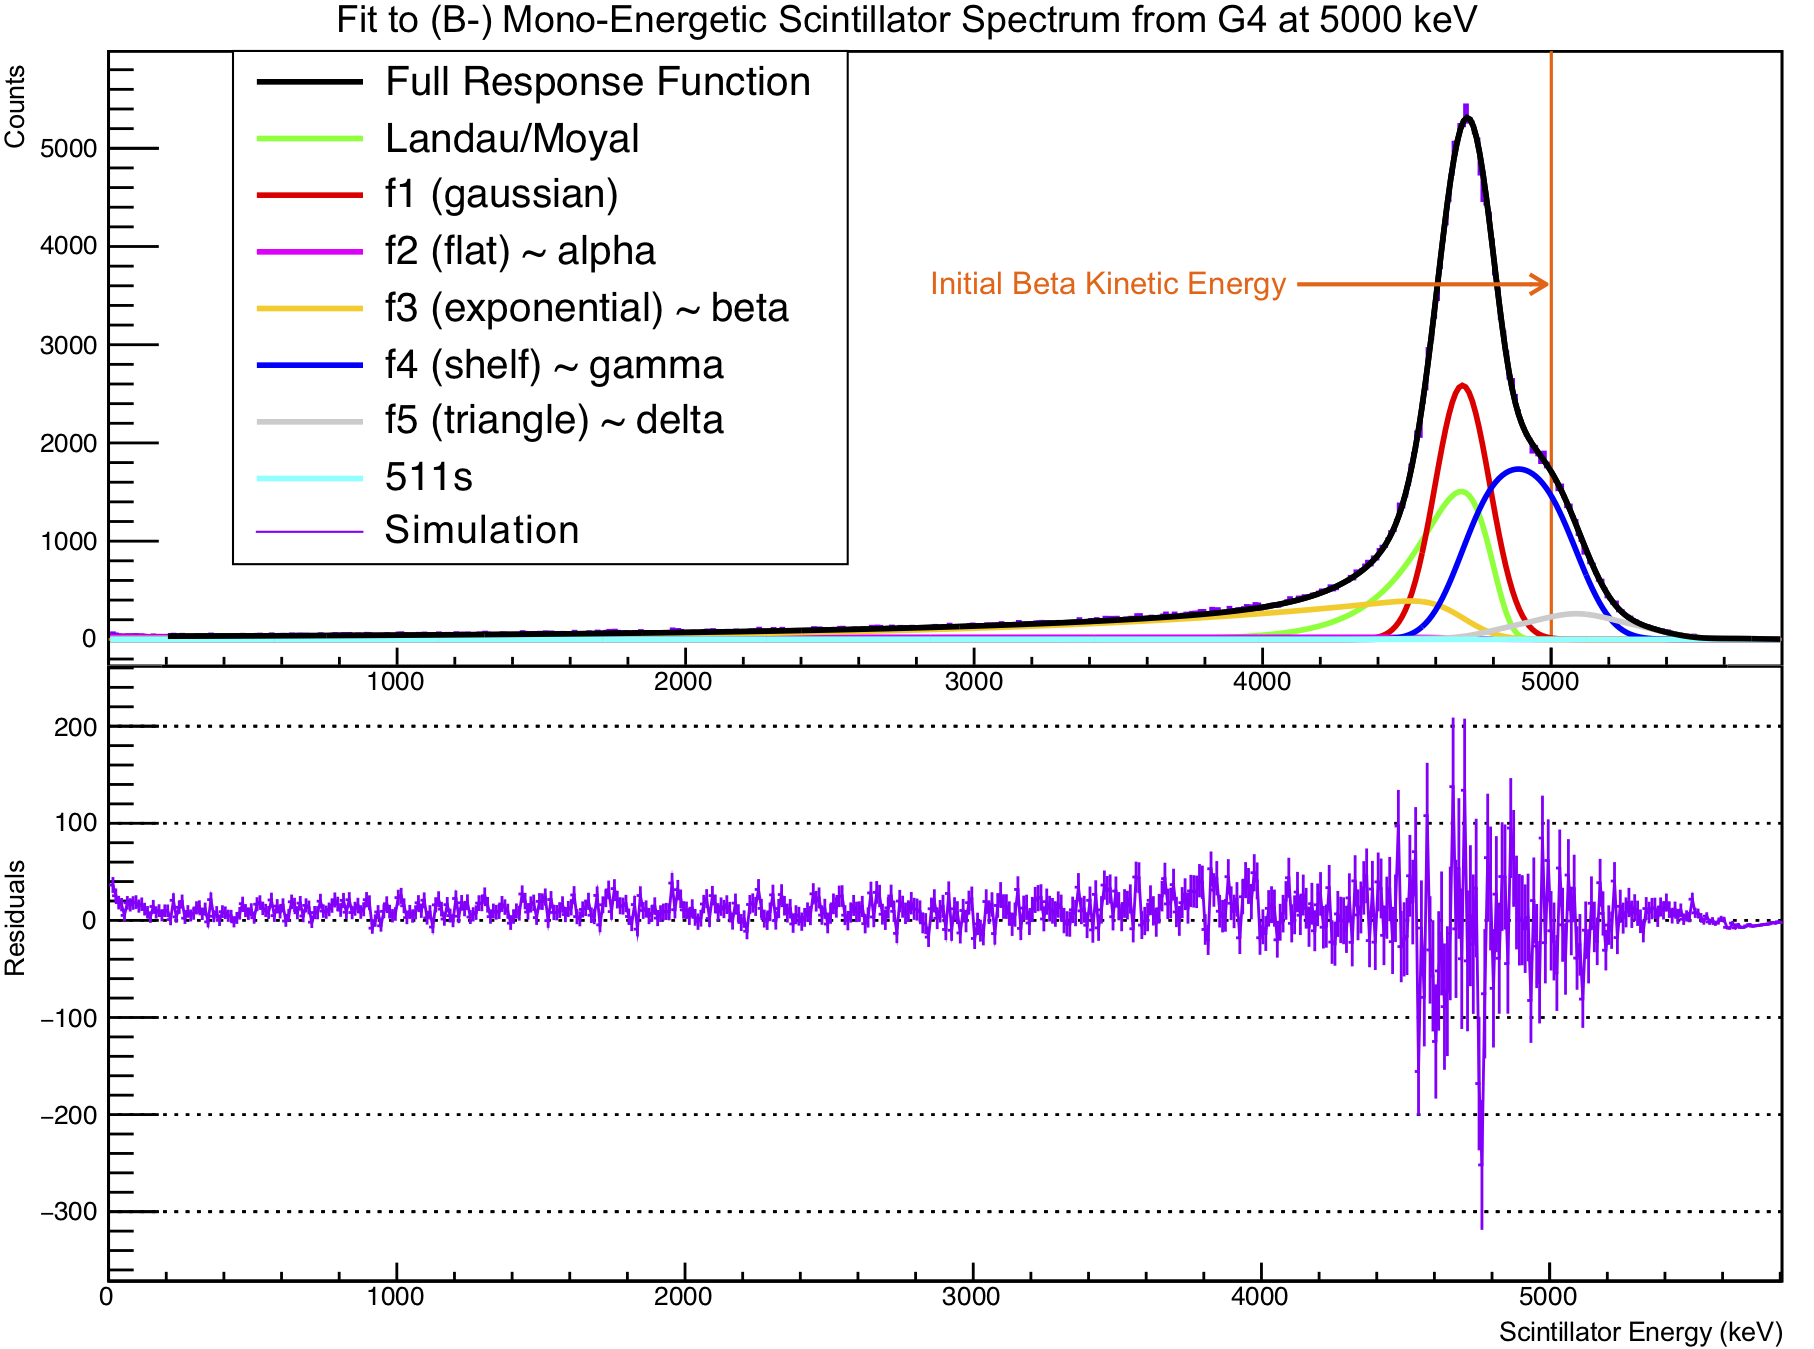
\includegraphics[width=.999\linewidth]
	{Figures/MonoFit_5000.png}
	\caption[Fit to Mono-Energetic Spectrum, 5000 keV]{Fit to Mono-Energetic Spectrum, 5000 keV (B-)}	
	\label{fig:lineshape_5000}
\end{figure}
\begin{figure}[h!!tb]
	\centering
	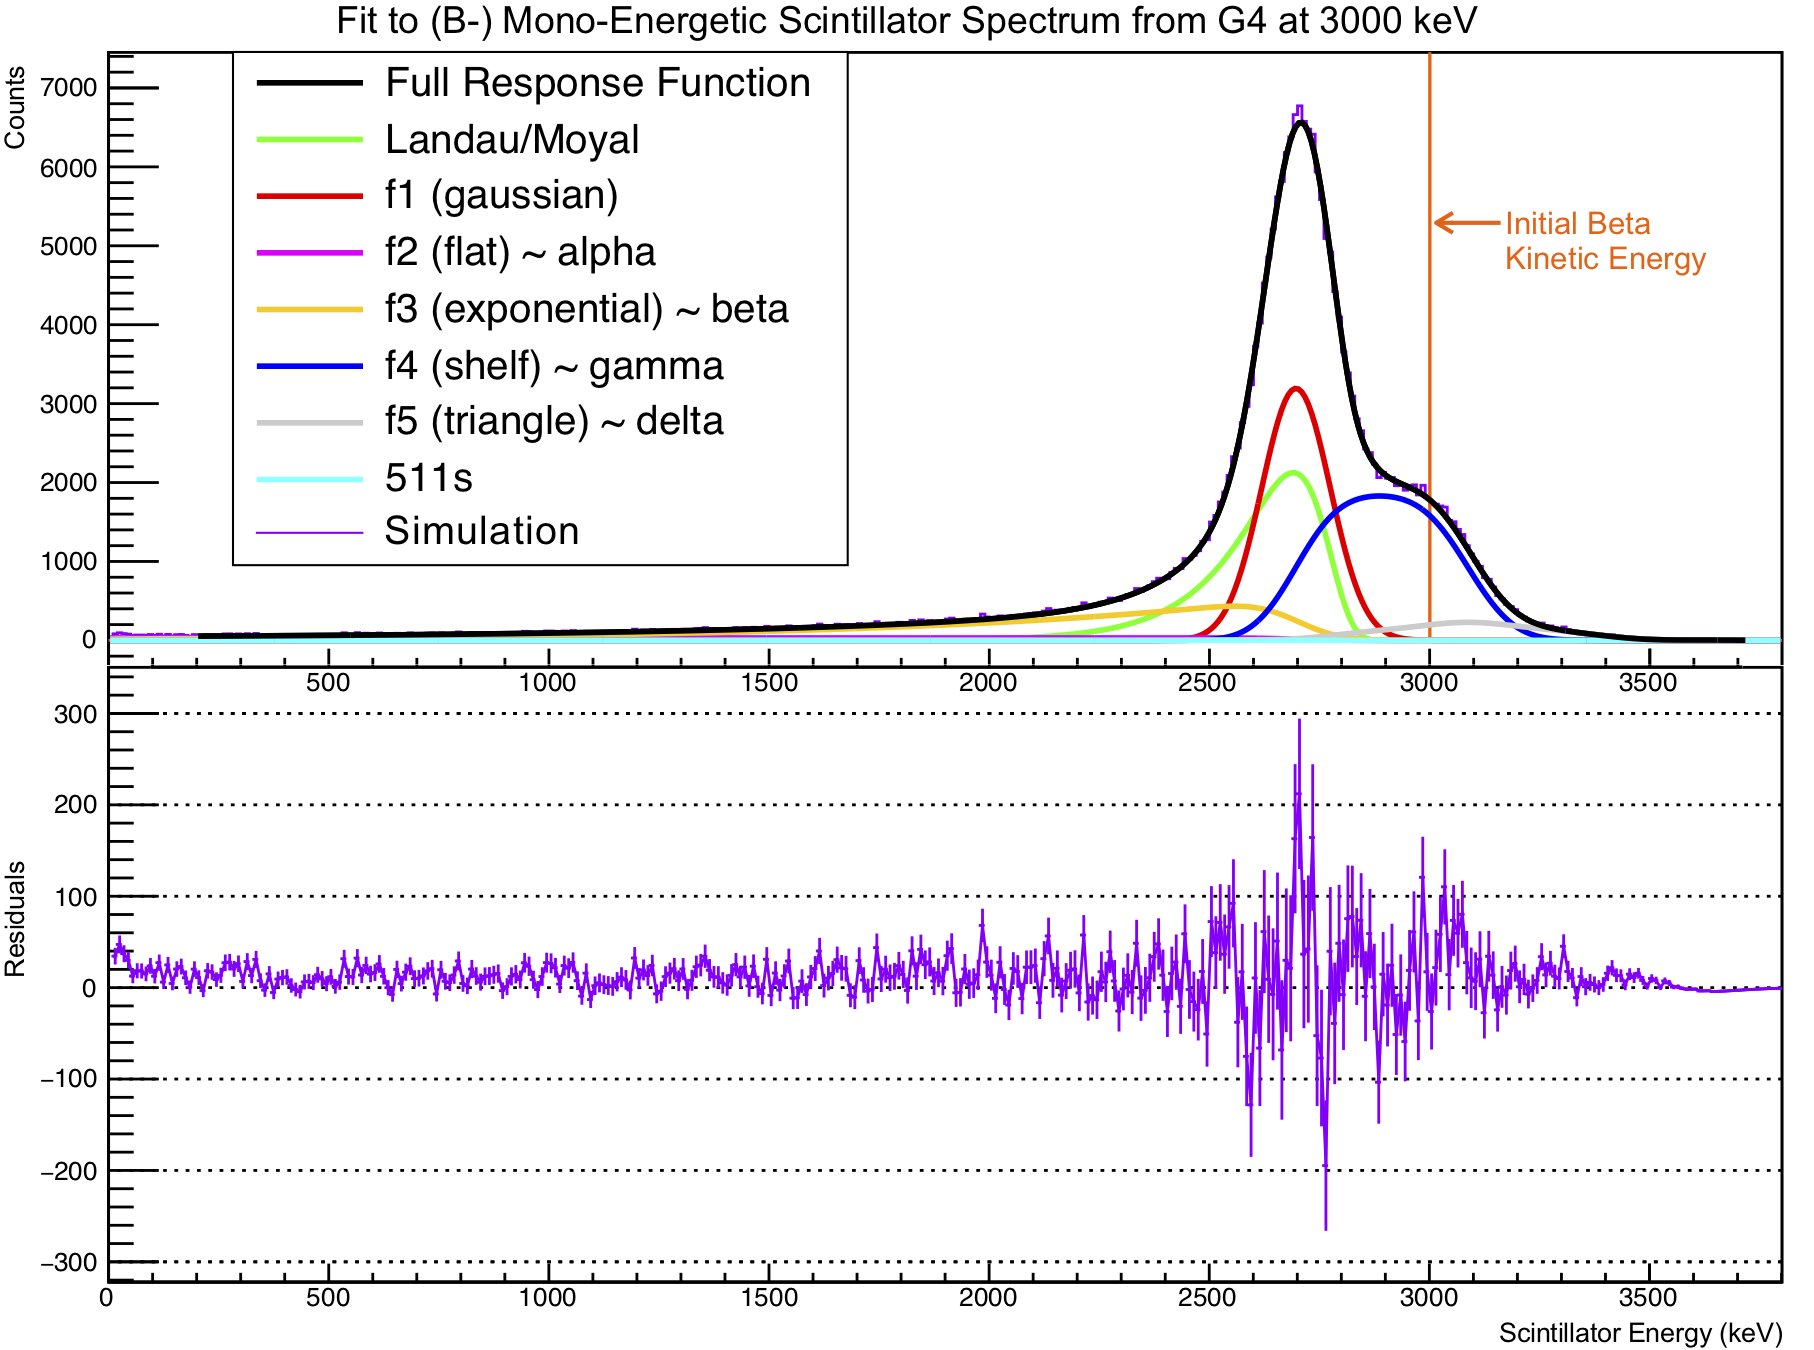
\includegraphics[width=.999\linewidth]
	{Figures/MonoFit_3000.png}
	\caption[Fit to Mono-Energetic Spectrum, 3000 keV]{Fit to Mono-Energetic Spectrum, 3000 keV (B-)}	
	\label{fig:lineshape_3000}
\end{figure}
\begin{figure}[h!!tb]
	\centering
	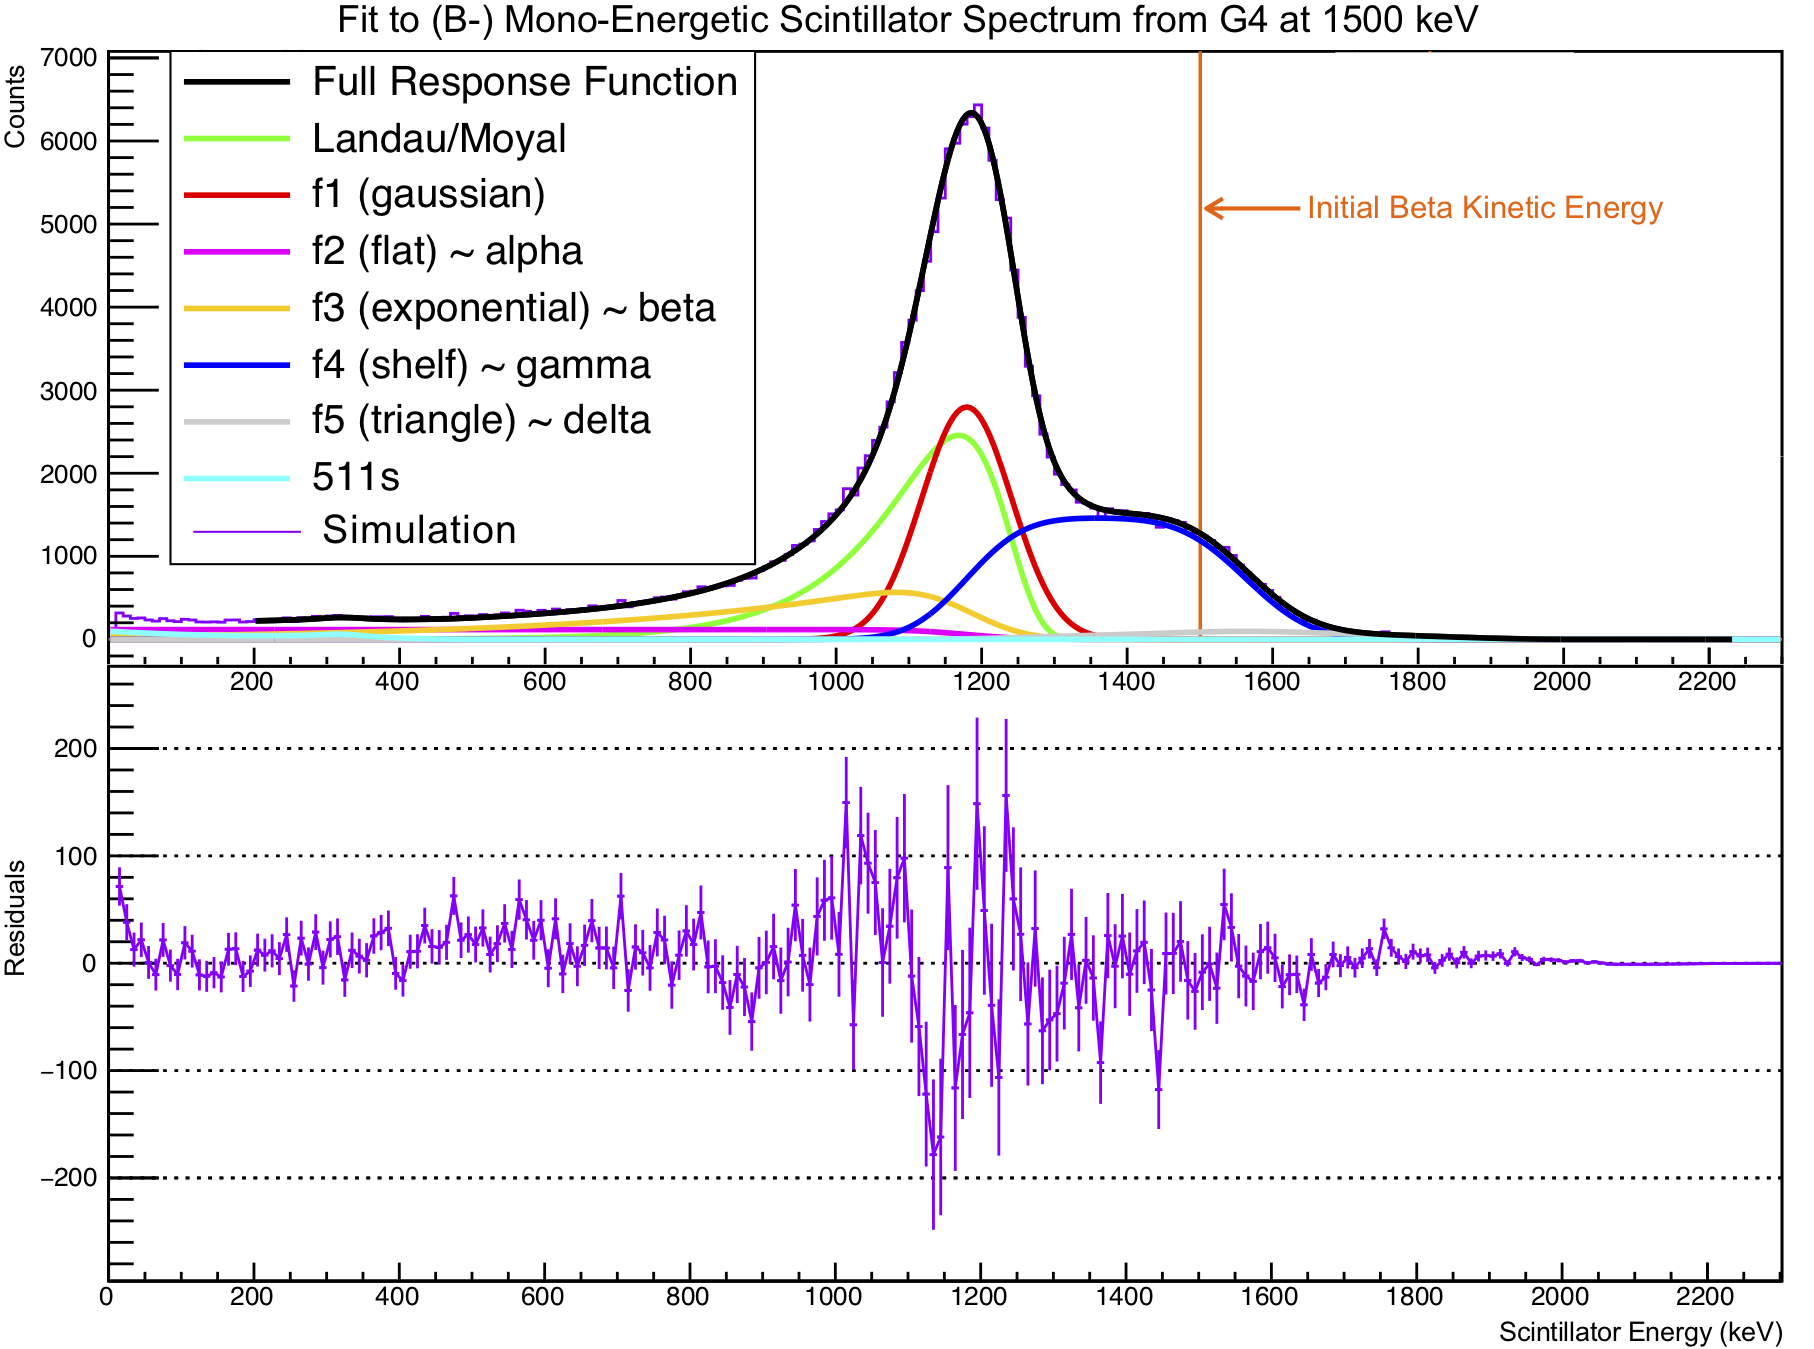
\includegraphics[width=.999\linewidth]
	{Figures/MonoFit_1500.png}
	\caption[Fit to Mono-Energetic Spectrum, 1500 keV]{Fit to Mono-Energetic Spectrum, 1500 keV (B-)}	
	\label{fig:lineshape_1500}
\end{figure}
\begin{figure}[h!!tb]
	\centering
	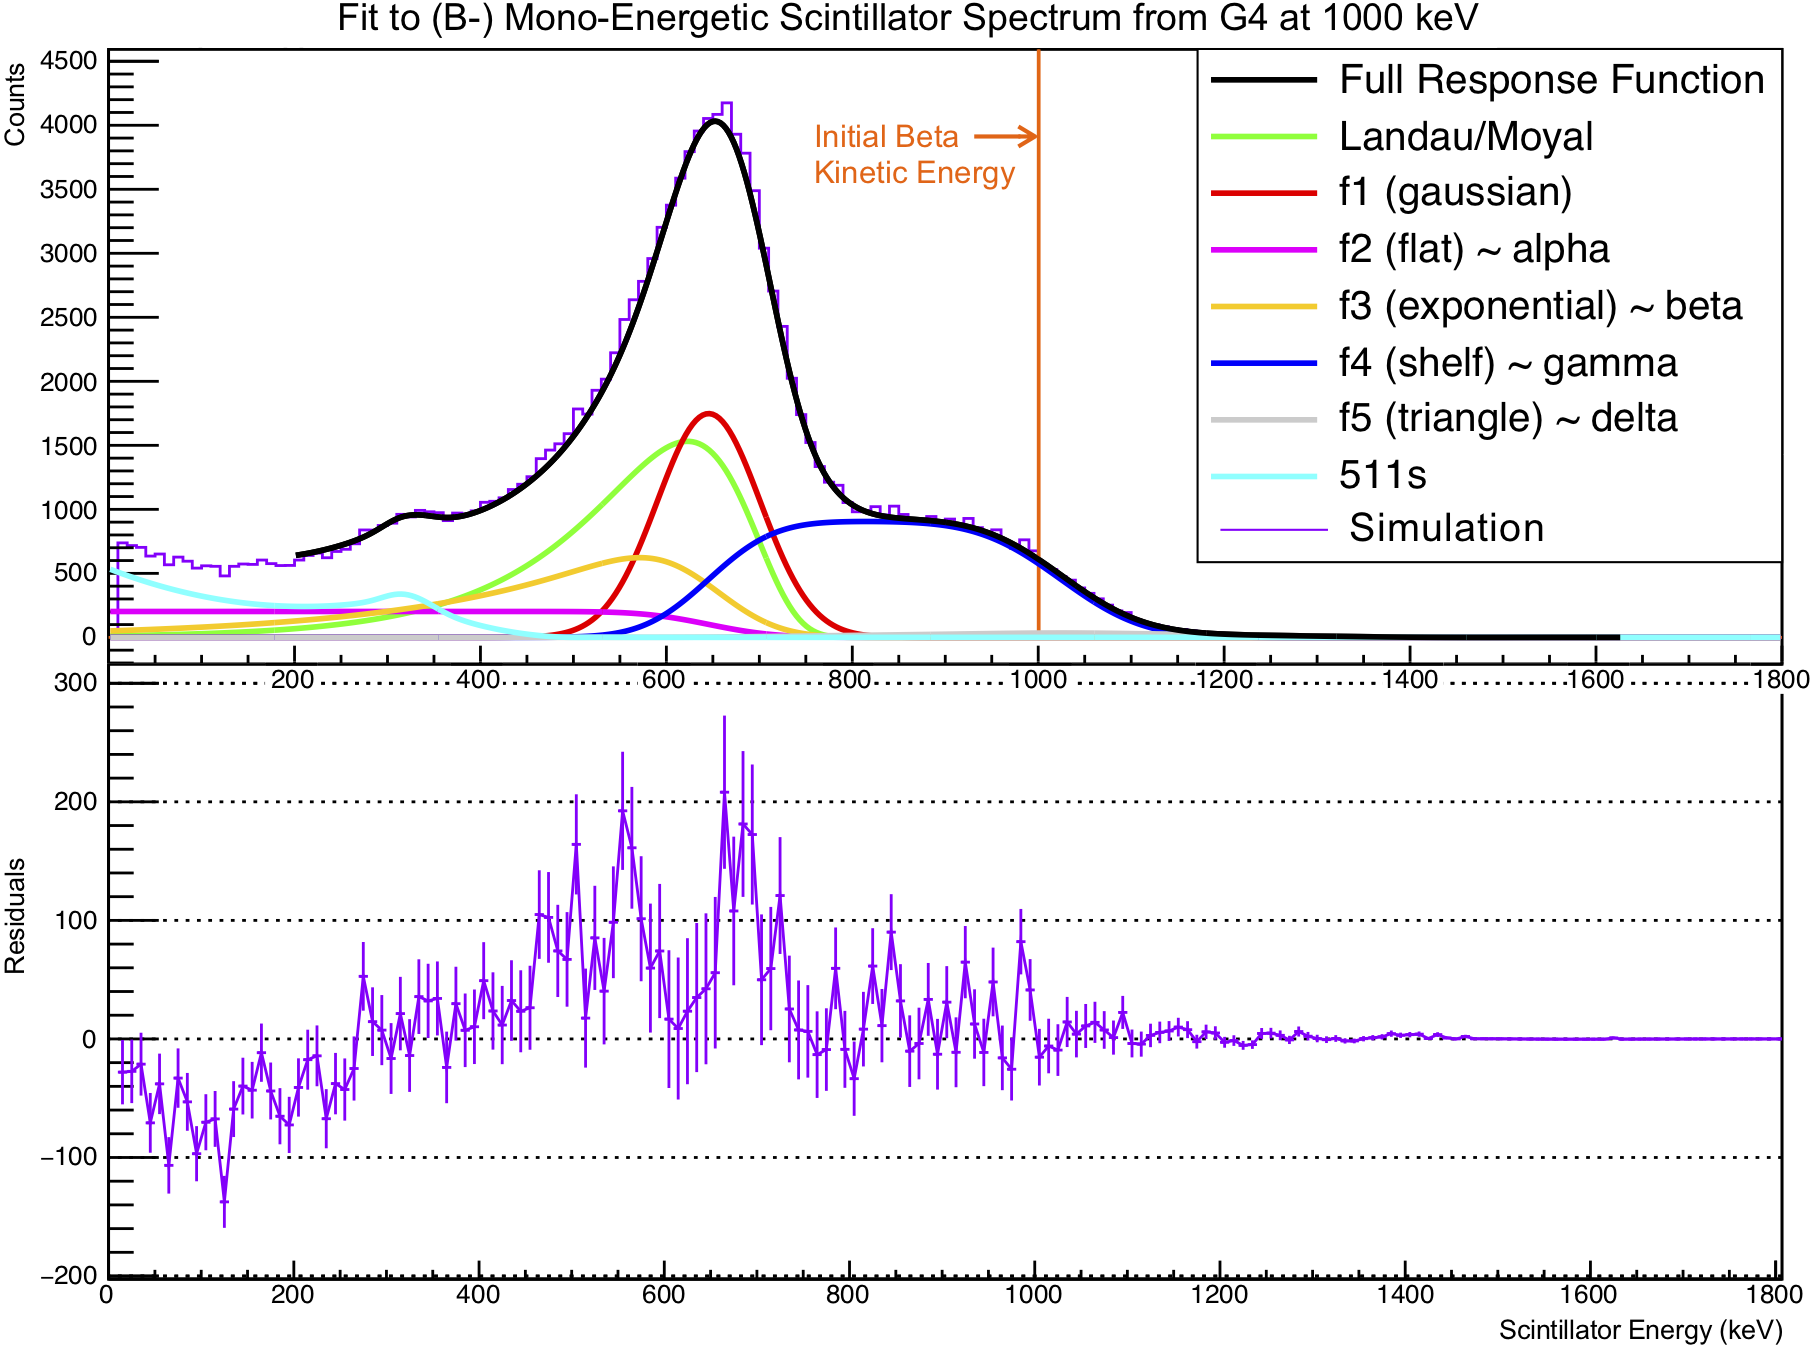
\includegraphics[width=.999\linewidth]
	{Figures/MonoFit_1000.png}
	\caption[Fit to Mono-Energetic Spectrum, 1000 keV]{Fit to Mono-Energetic Spectrum, 1000 keV (B-)}	
	\label{fig:lineshape_1000}
\end{figure}
\begin{figure}[h!!tb]
	\centering
	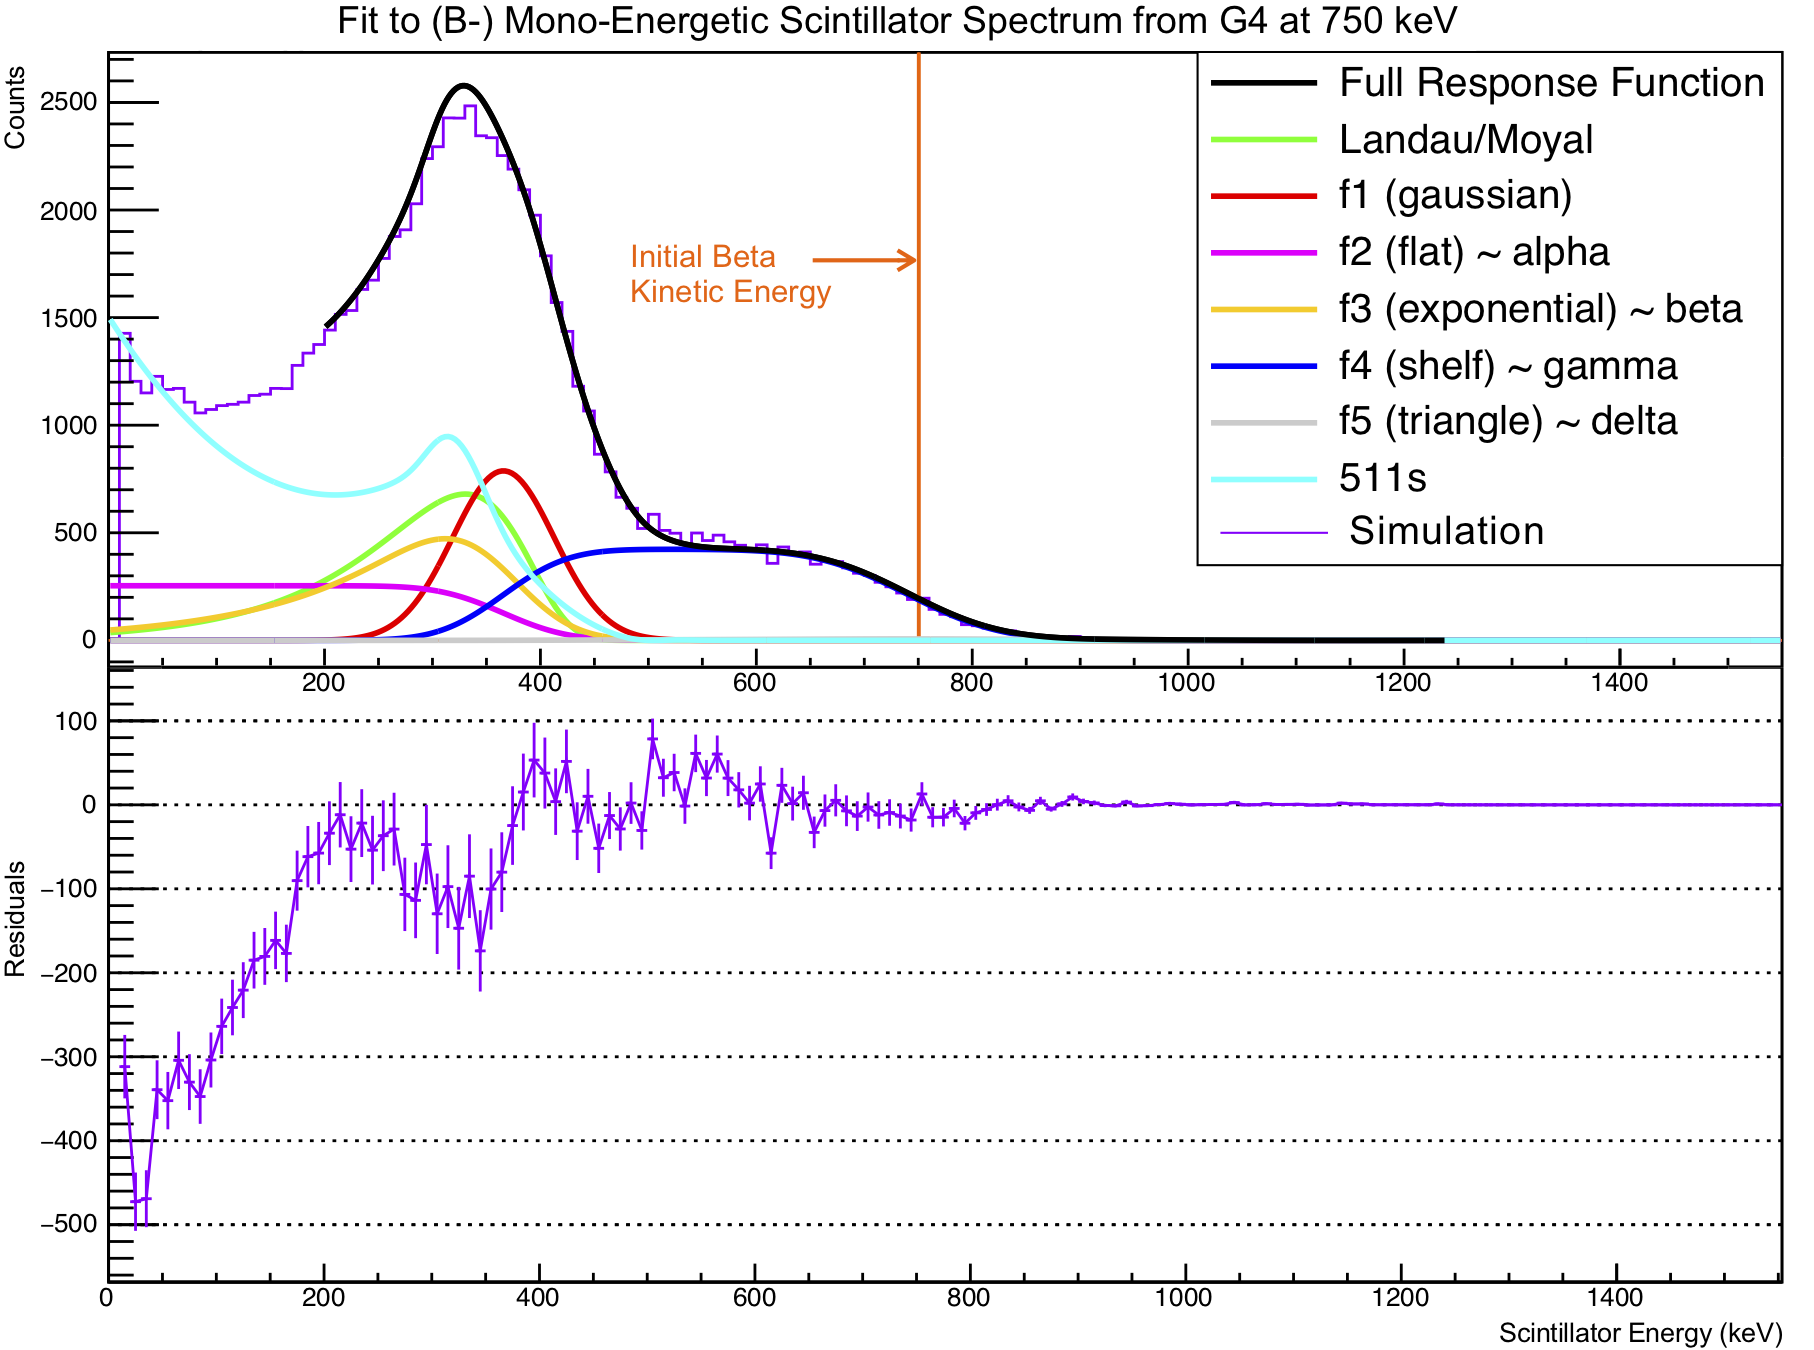
\includegraphics[width=.999\linewidth]
	{Figures/MonoFit_750.png}
	\caption[Fit to Mono-Energetic Spectrum, 750 keV]{Fit to Mono-Energetic Spectrum, 750 keV (B-)}	
	\label{fig:lineshape_750}
\end{figure}
%\FloatBarrier  % this will have to go in the end, but it's really hard to edit this thing without it.

The values of the individual parameters contributing to the fit functions in, eg, Figs.~\ref{fig:lineshape_5000},~\ref{fig:lineshape_3000},~\ref{fig:lineshape_1500},~\ref{fig:lineshape_1000}, and~\ref{fig:lineshape_750} are allowed to vary with initial beta energy, and the energy dependence of each parameter must be modeled in order to extrapolate the shape of the response function to intermediate initial beta kinetic energy values that are not explicitly modeled.  For each parameter, the energy dependence is modeled by an analytic function selected to have similar characteristics.  Each of these analytic functions is itself a function of several parameters which can be adjusted to optimize its fit to the true best-fit energy dependence of the parameter it models.  Because some parameters are only weakly independent, it is necessary to perform these fits iteratively on only a single parameter at a time, revisiting earlier parameter fits after fixing other parameters to updated models.  The results of this process are shown in Figs.~\ref{fig:lineshapeparams_part1}, ~\ref{fig:lineshapeparams_part2}, ~\ref{fig:lineshapeparams_part3}, and~\ref{fig:lineshapeparams_part4}.

\begin{figure}[h!!tb]
	\centering
	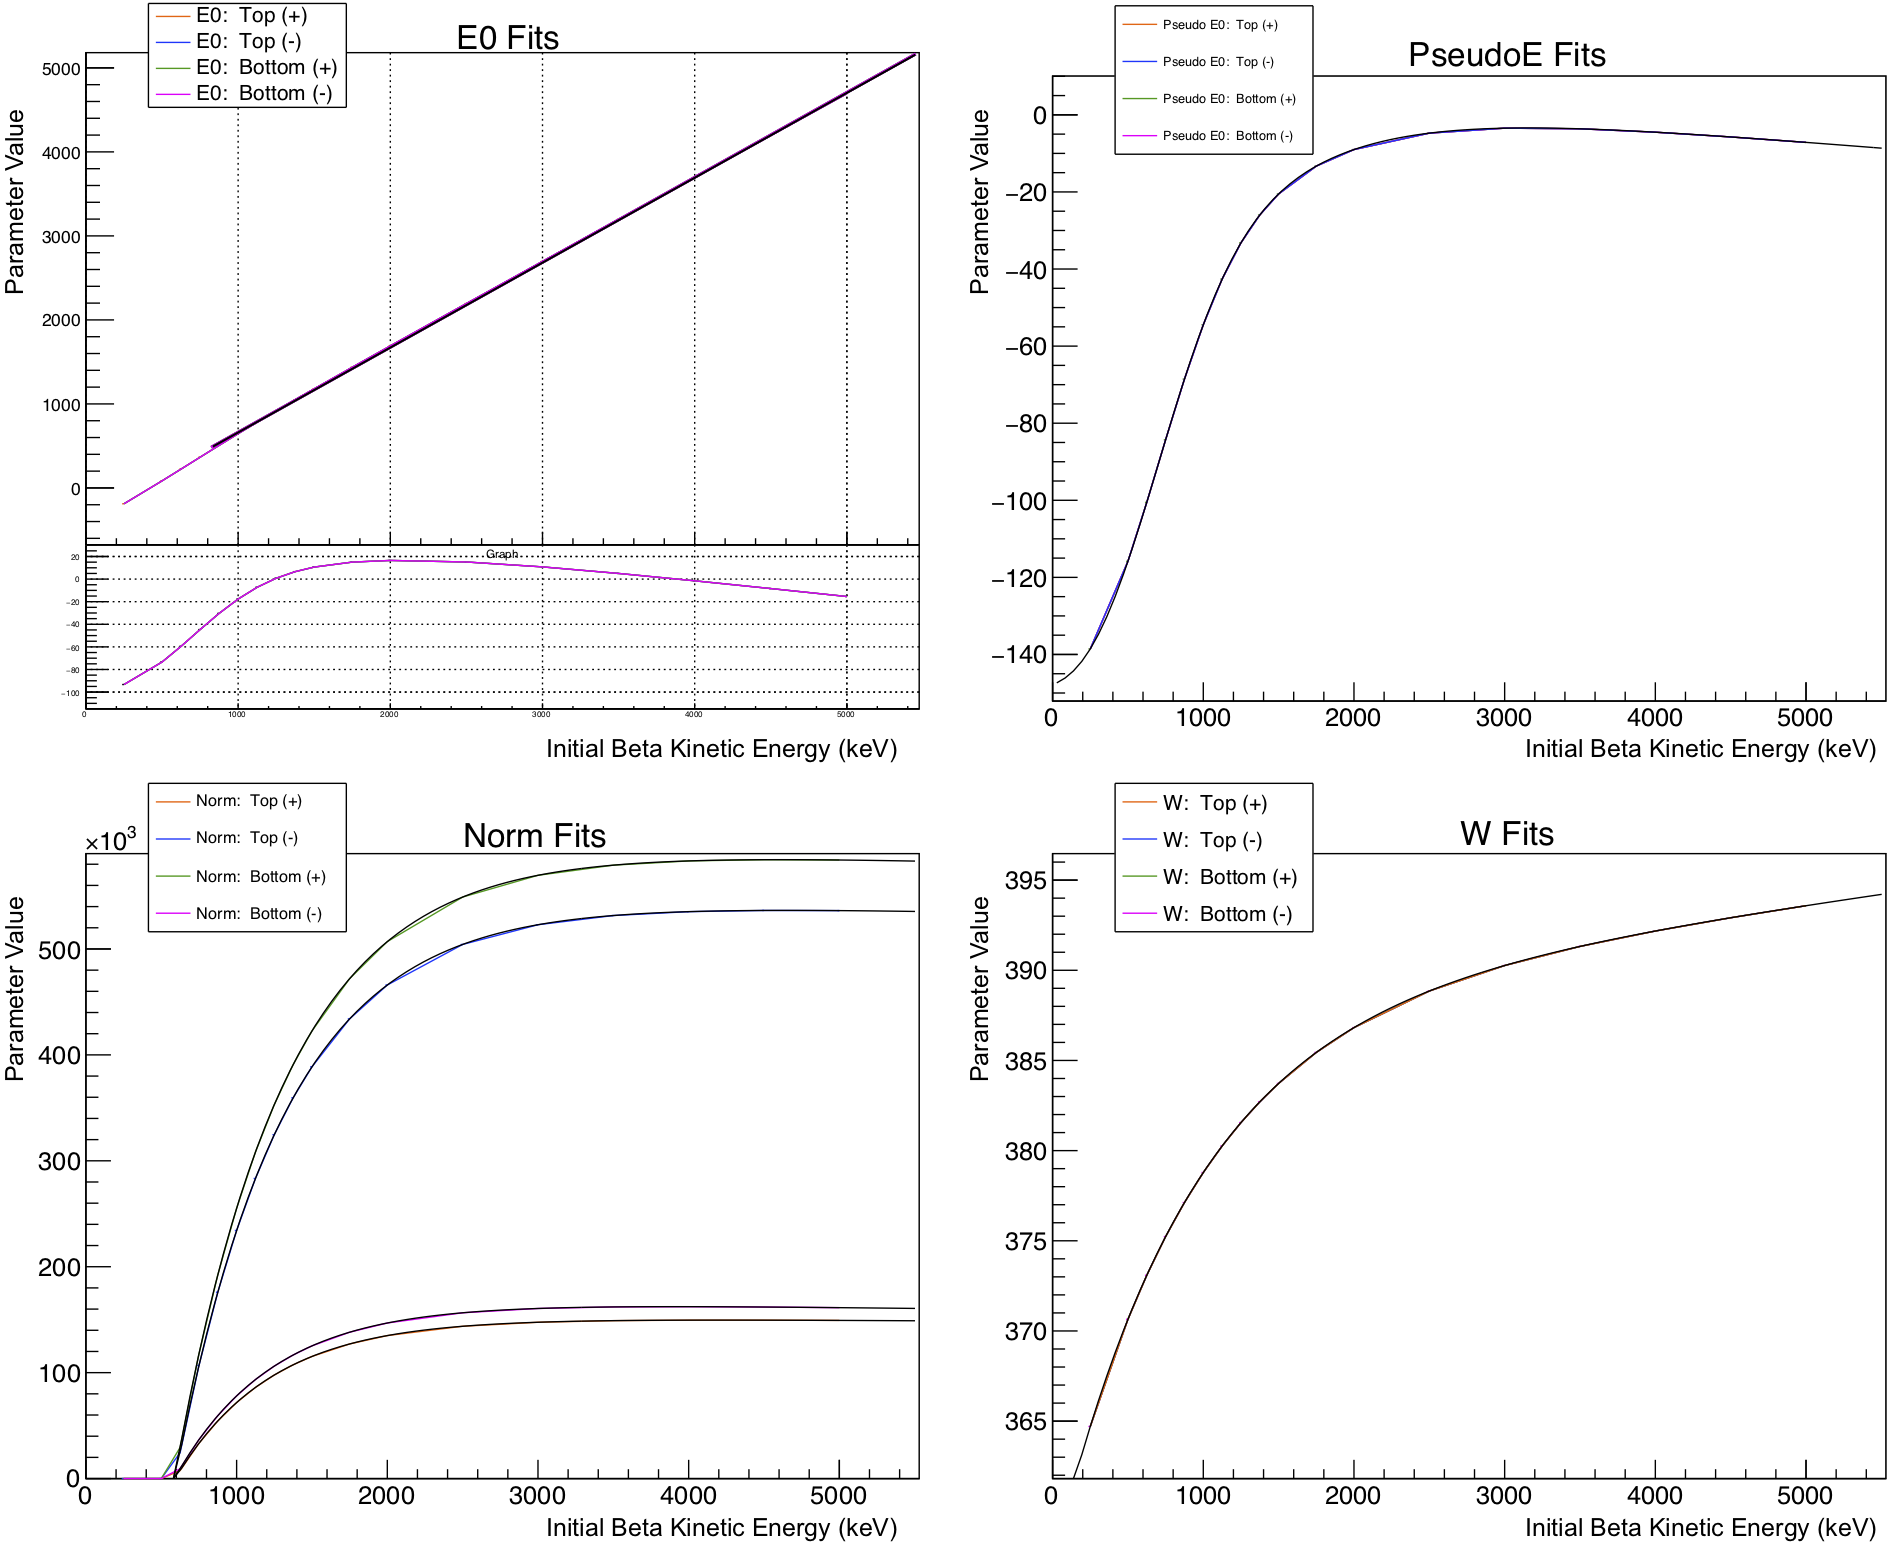
\includegraphics[width=.999\linewidth]
	{Figures/LineshapeParams_part1.png}
	\note[color=done]{What even \emph{is} the thing plotted below E0 in the `residuals' spot, you ask?  It's `PseudoE', which is describes the difference between the original input energy, $E_0$, and the energy where the output spectrum is maximal. Or something.  To `pretty good' order, it's a straight line.  the `PseudoE' plot shows what's left after you fit it to a straight line.  It's fucking weird that it's negative everywhere.  Like, what?}
	\caption[Lineshape Parameter Fits (Part 1)]{Lineshape Parameter Fits (Part 1)}	
	\label{fig:lineshapeparams_part1}
\end{figure}
\begin{figure}[h!!tb]
	\centering
	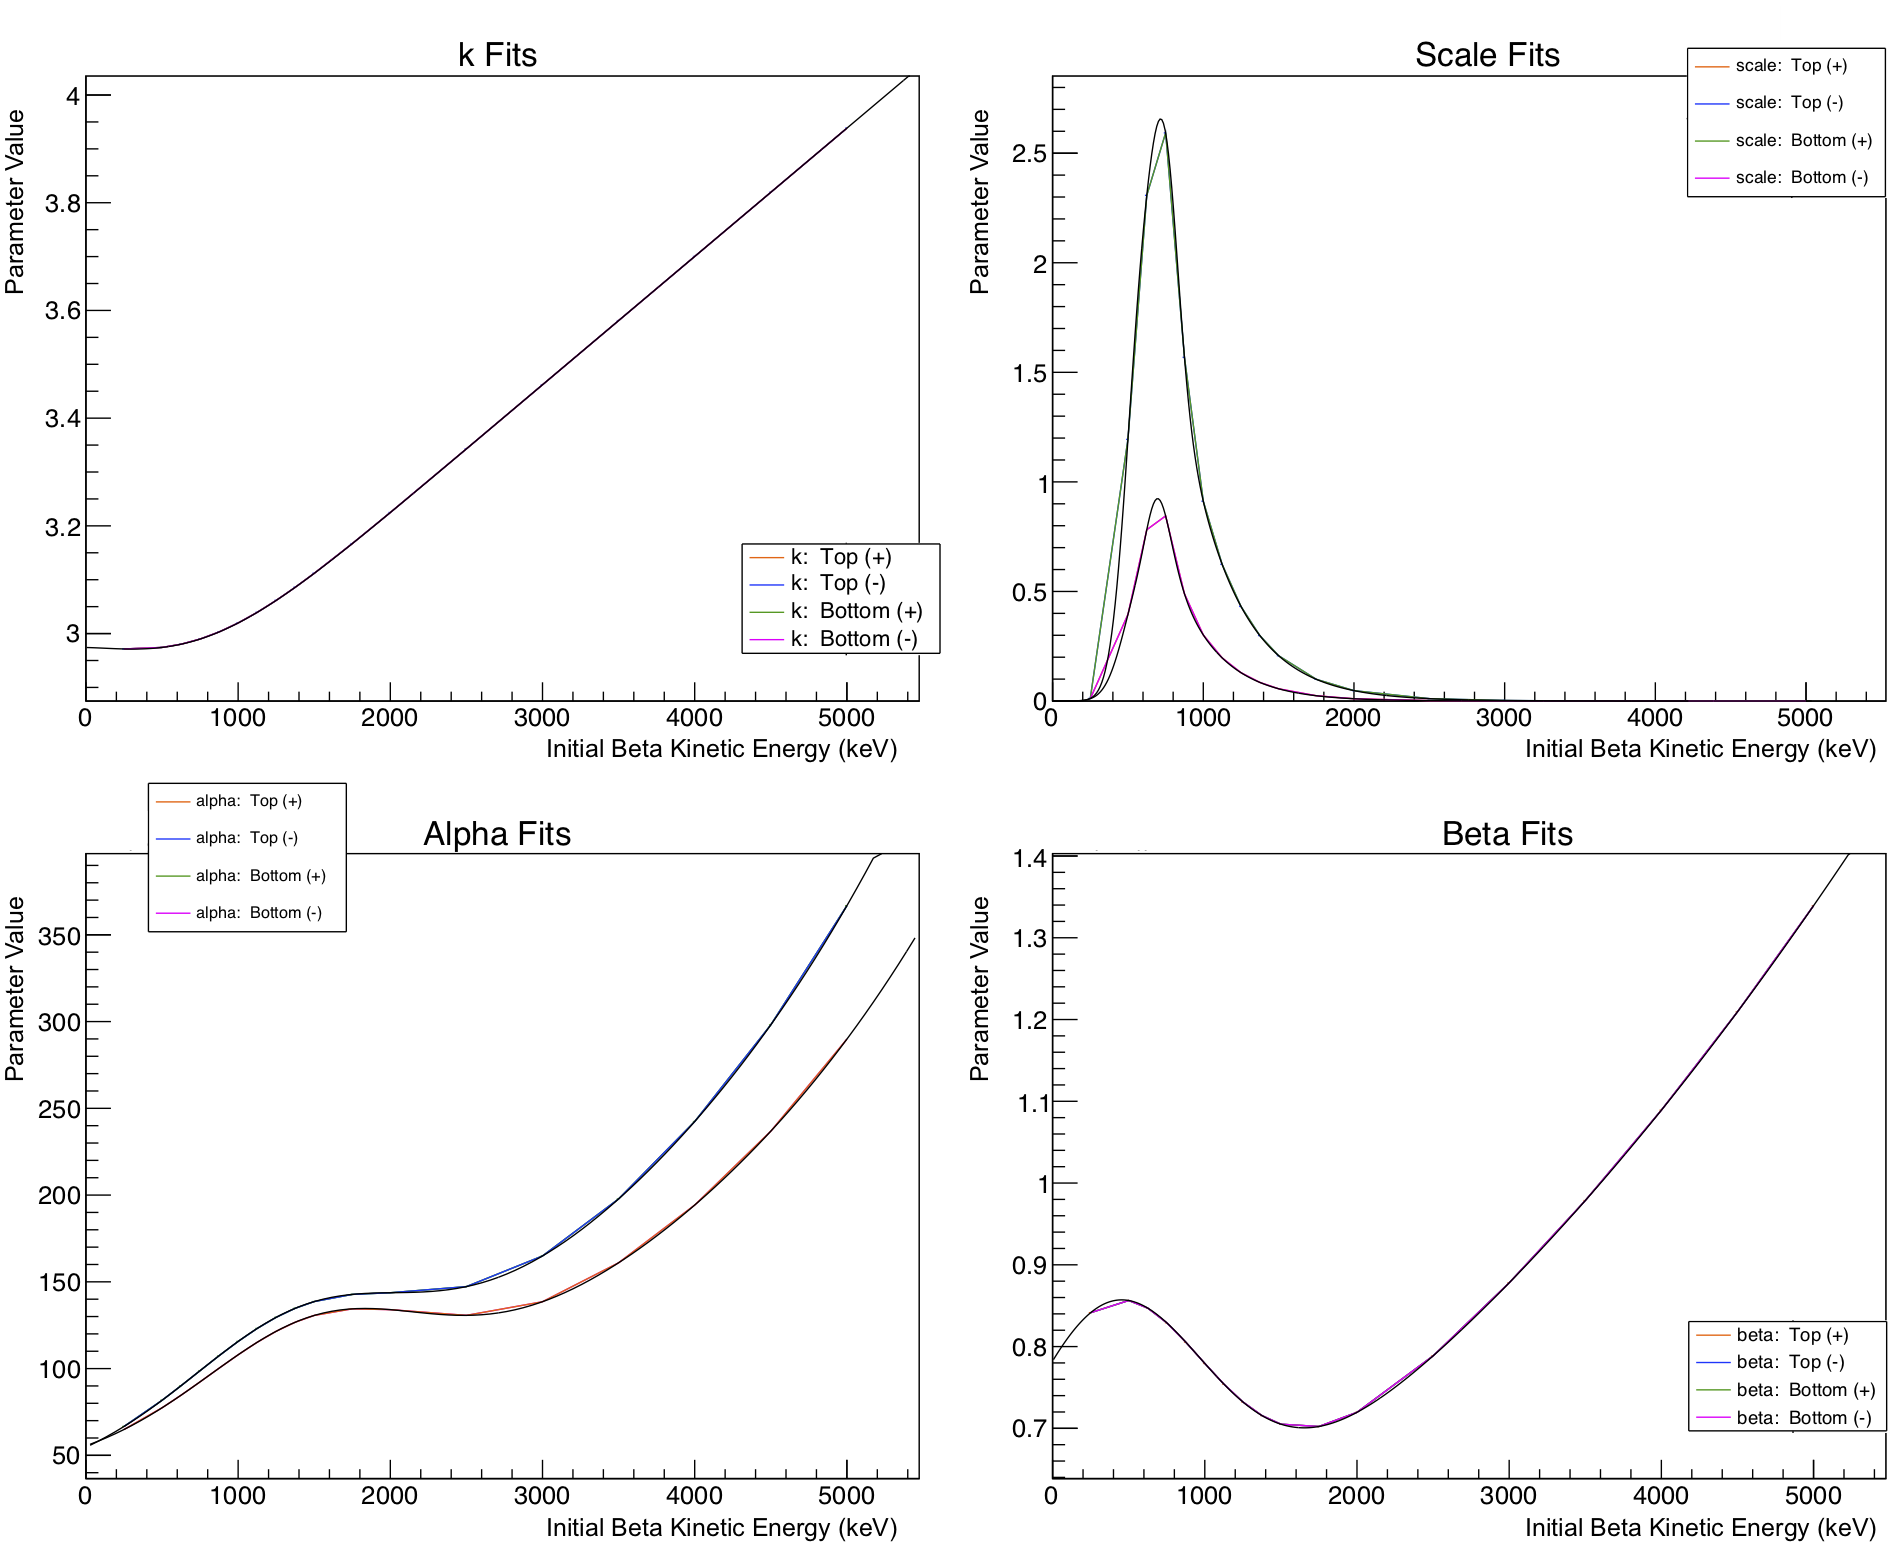
\includegraphics[width=.999\linewidth]
	{Figures/LineshapeParams_part2.png}
	\caption[Lineshape Parameter Fits (Part 2)]{Lineshape Parameter Fits (Part 2)}
	\label{fig:lineshapeparams_scale}
	\label{fig:lineshapeparams_part2}
\end{figure}
\begin{figure}[h!!tb]
	\centering
	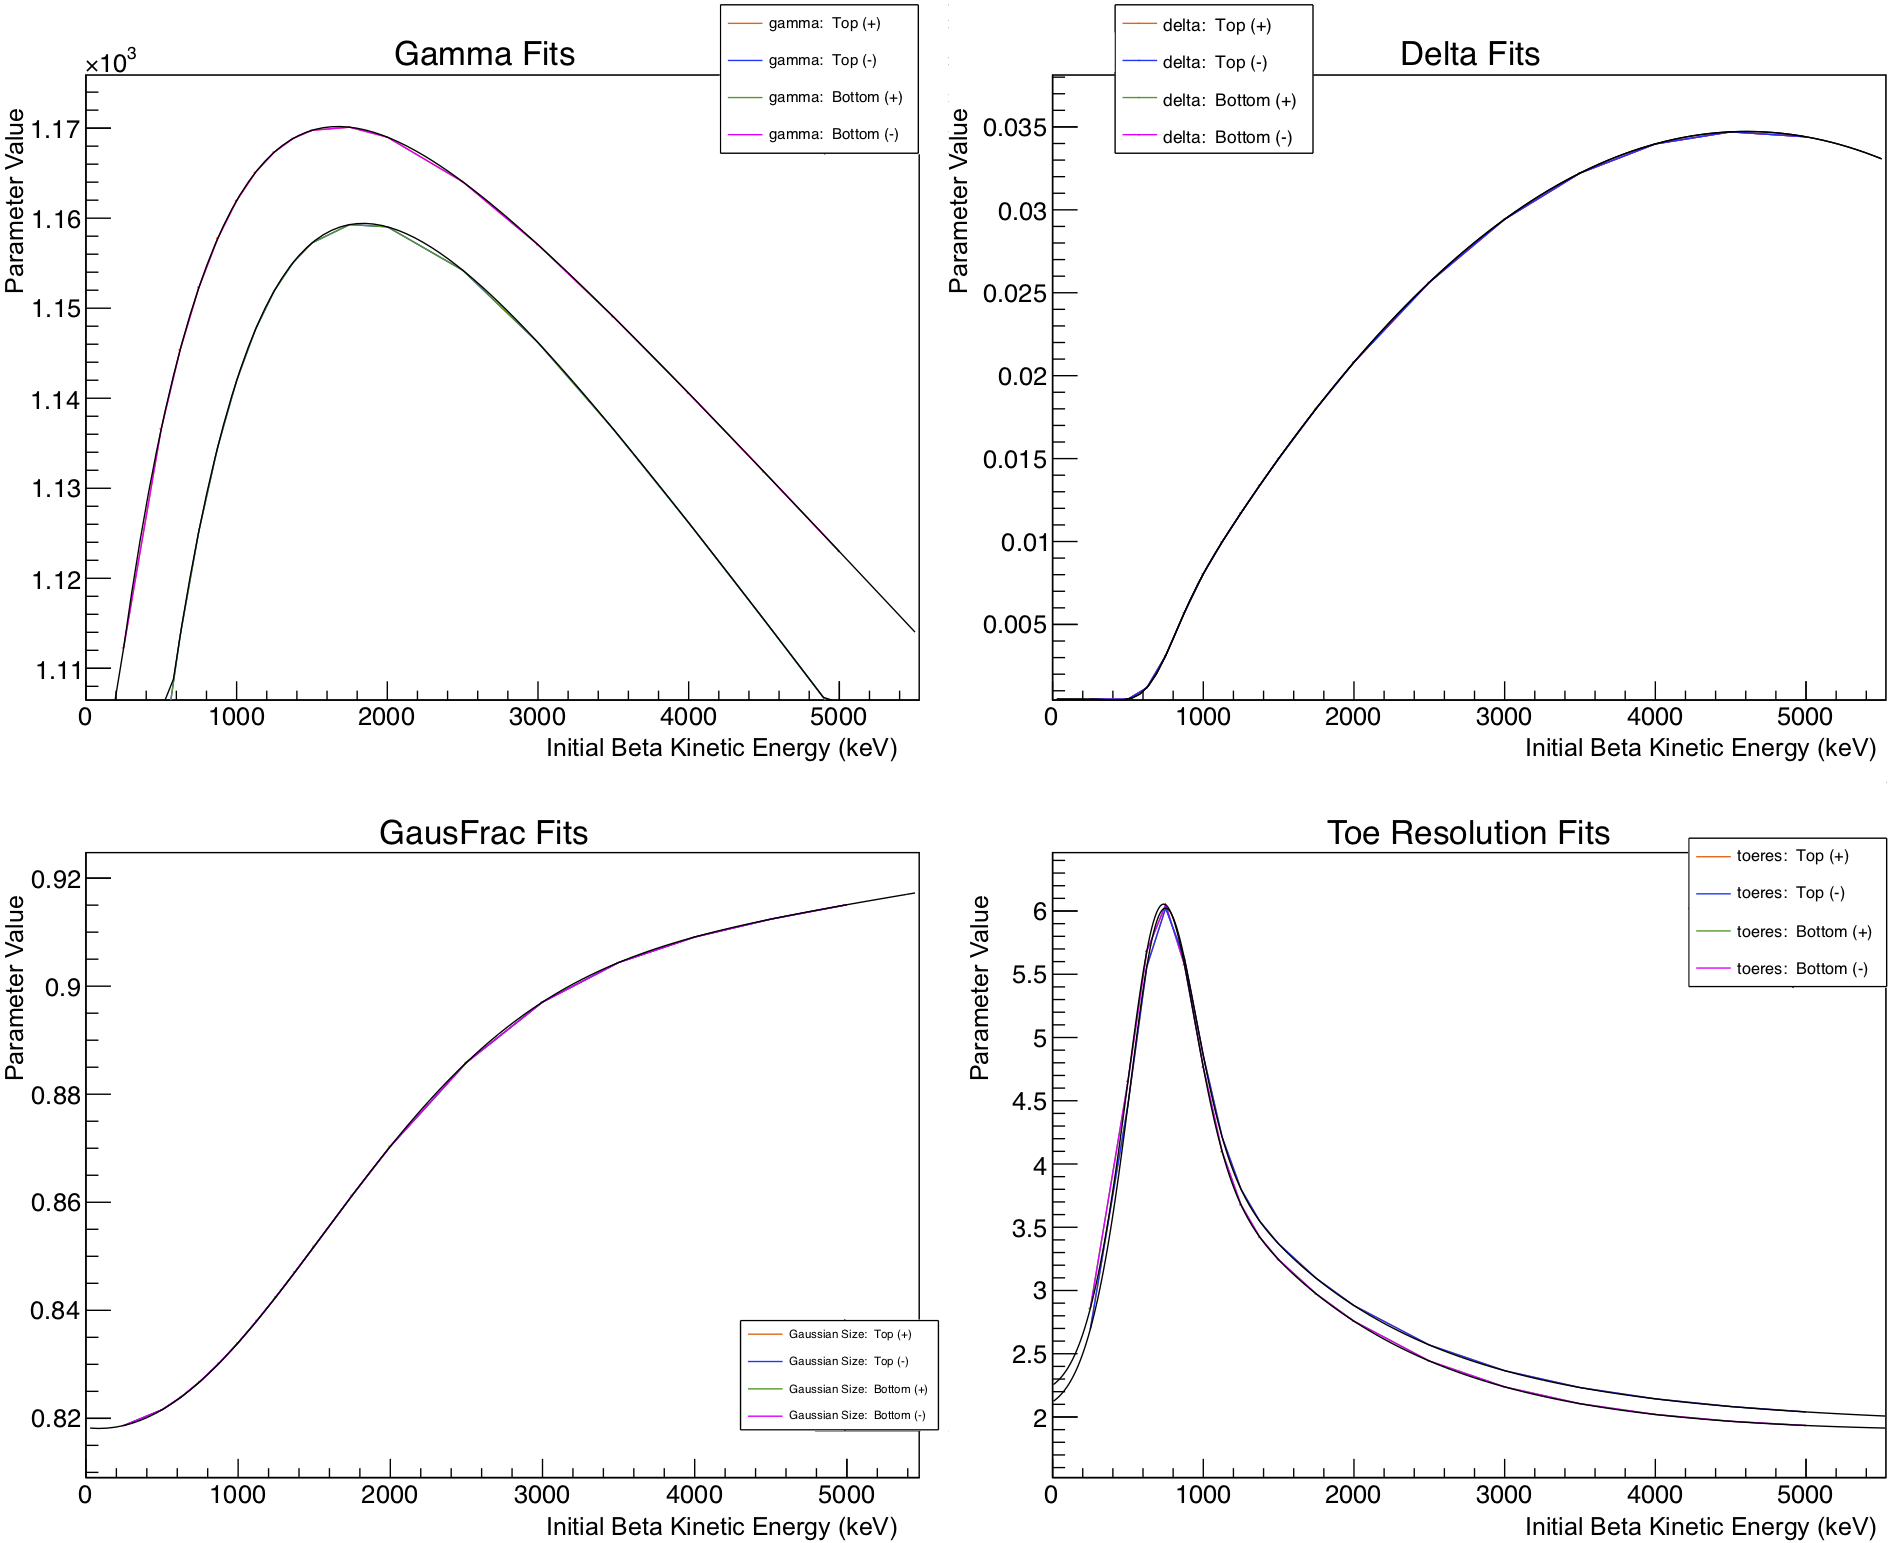
\includegraphics[width=.999\linewidth]
	{Figures/LineshapeParams_part3.png}
	\caption[Lineshape Parameter Fits (Part 3)]{Lineshape Parameter Fits (Part 3)}	
	\label{fig:lineshapeparams_part3}
\end{figure}
\begin{figure}[h!!tb]
	\centering
	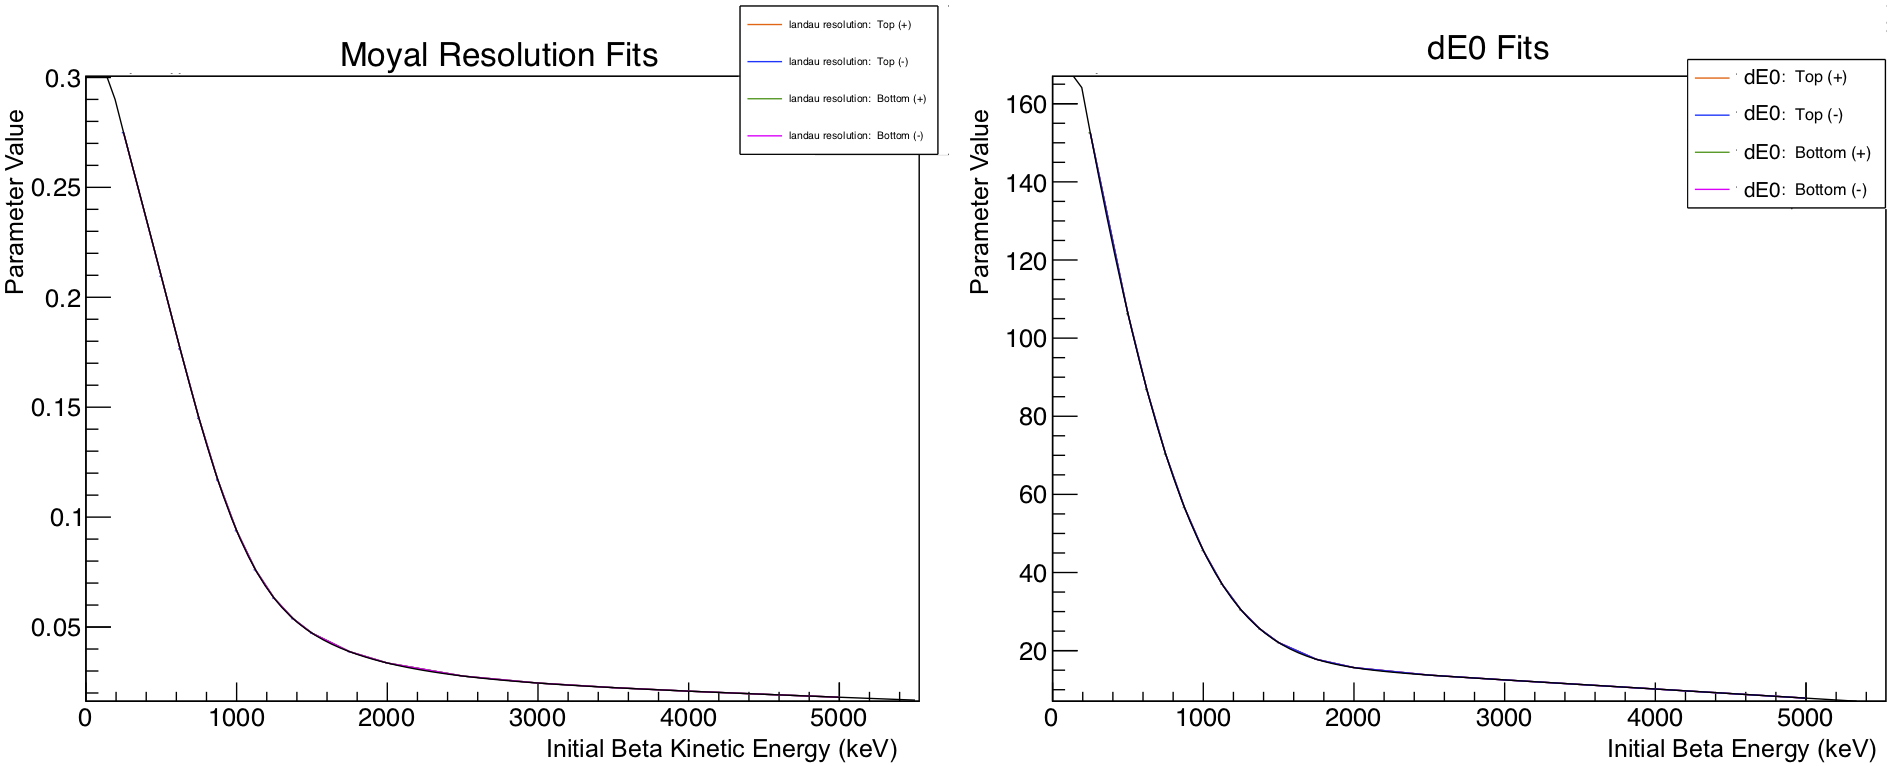
\includegraphics[width=.999\linewidth]
	{Figures/LineshapeParams_part4.png}
	\caption[Lineshape Parameter Fits (Part 4)]{Lineshape Parameter Fits (Part 4)}	
	\label{fig:lineshapeparams_part4}
\end{figure}
%
%\FloatBarrier  % this will have to go in the end, but it's really hard to edit this thing without it.
It is useful to consider how well this empirical response function works to model the spectra.  One can see clearly from Figs.~\ref{fig:lineshape_5000}, ~\ref{fig:lineshape_3000}, ~\ref{fig:lineshape_1500}, ~\ref{fig:lineshape_1000}, and~\ref{fig:lineshape_750} that the fit residuals appear noticeably \emph{worse} at lower initial beta energies.  Fig.~\ref{fig:lineshape_redchi2} shows the reduced $\chi^2$ values arising from comparing mono-energetic G4 spectra to the empirical response functions described above, for all four detector and polarization combinations.

\begin{figure}[h!!tb]
	\centering
	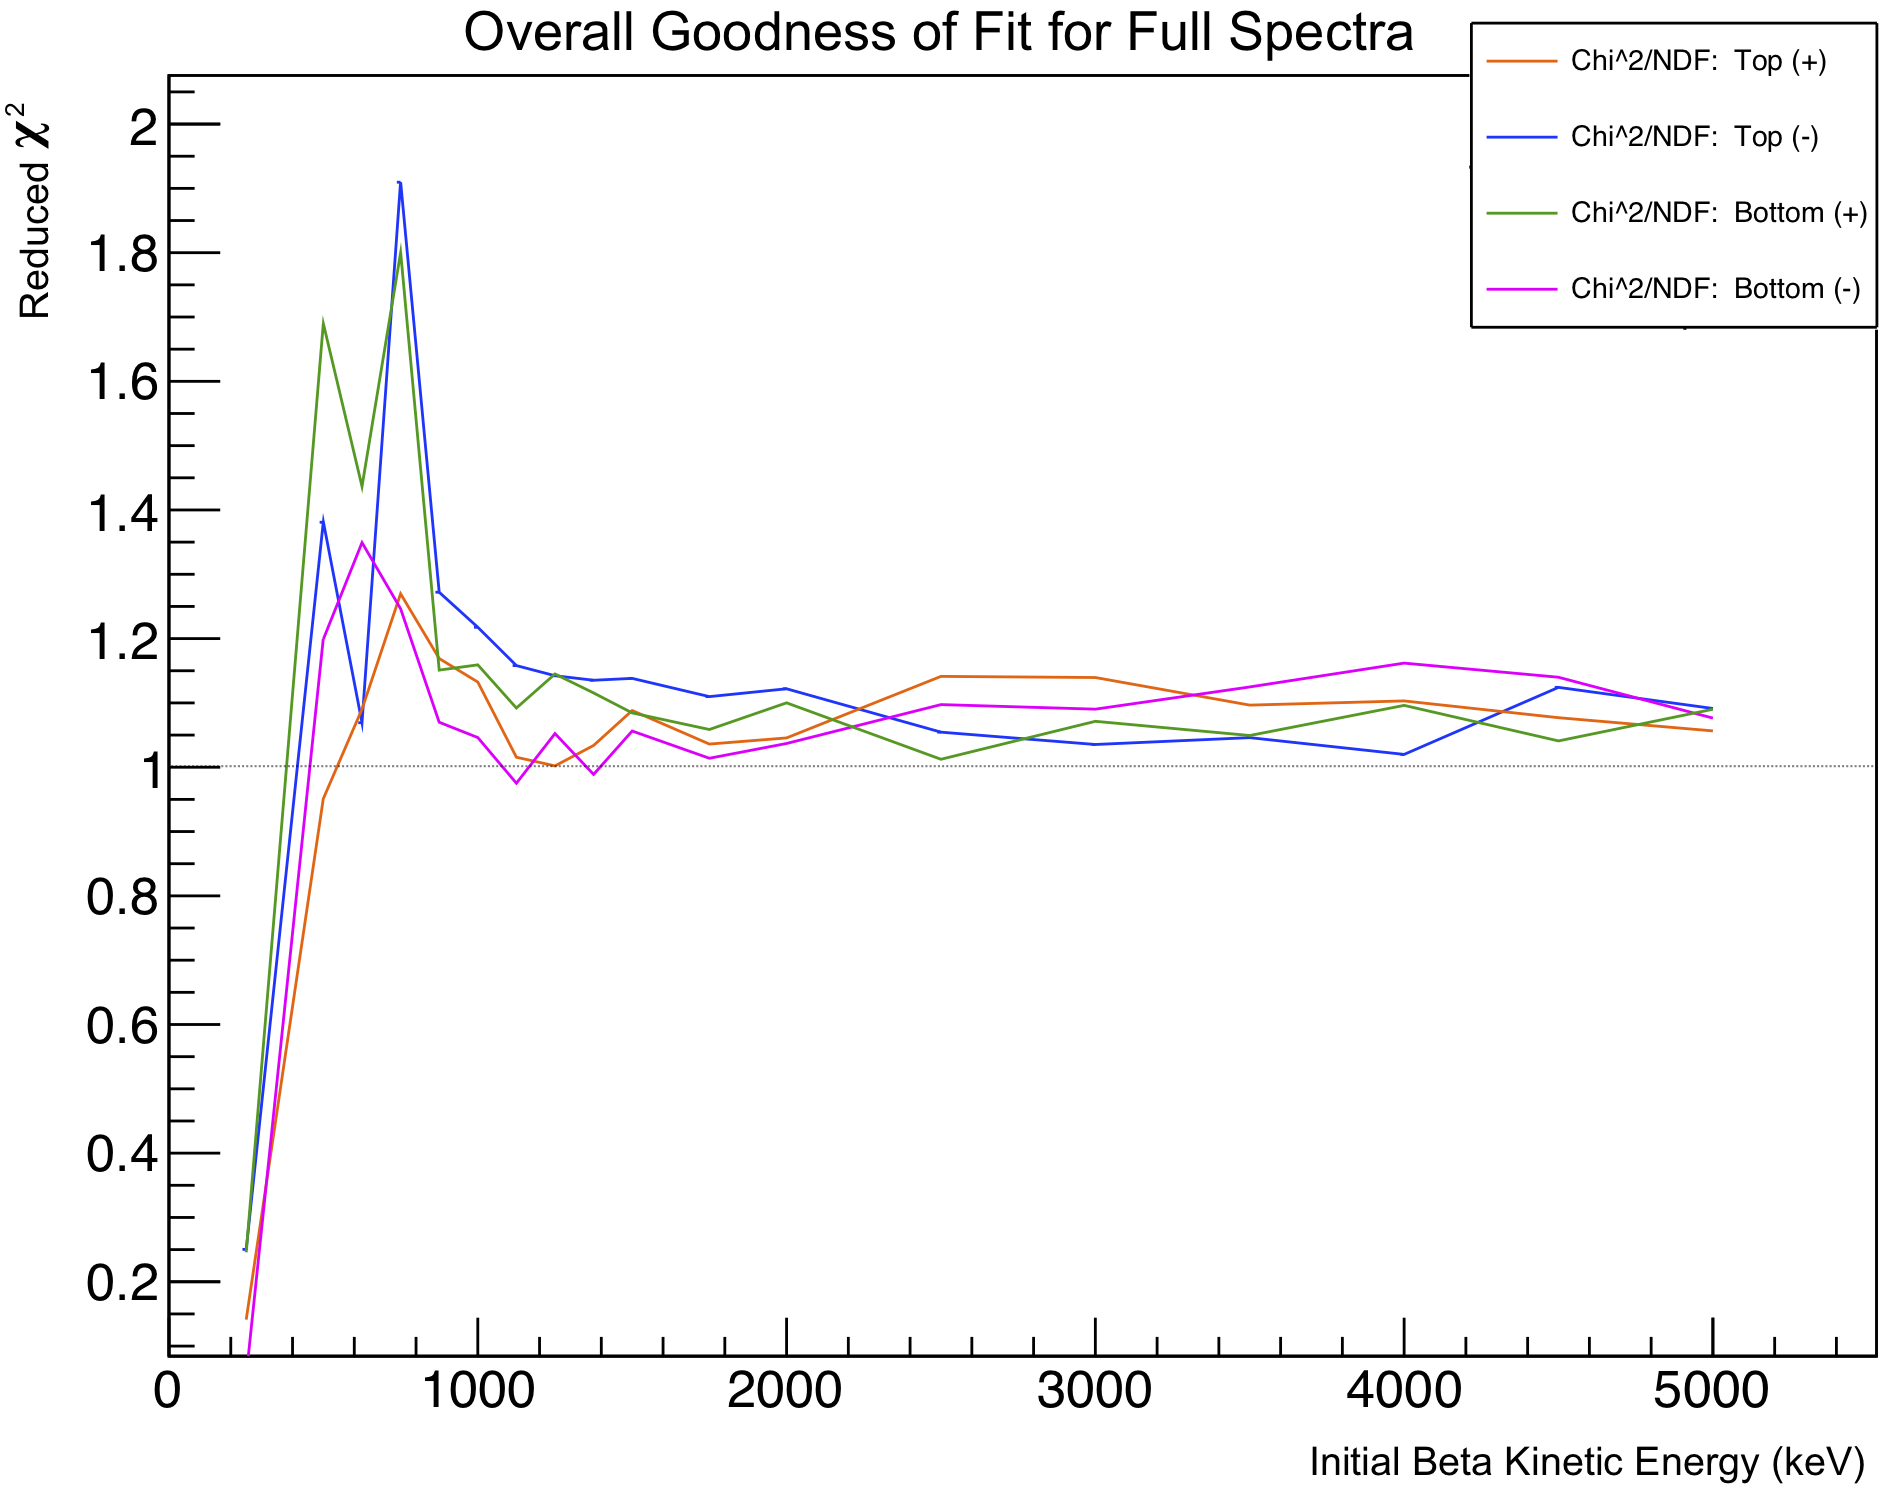
\includegraphics[width=.999\linewidth]
	{Figures/Lineshape_Chi2.png}
	\note{How many DOF for these things?  I should put it on the picture.}
	\caption[Goodness of Fit for Modeled Response Functions]{Goodness of fit for modeled response functions, for all four detector+polarization combinations.  The models are clearly much better behaved at initial energies above $\sim 1200\,$keV.}	
	\label{fig:lineshape_redchi2}
\end{figure}


With the energy dependence for each of the response function's parameters carefully modeled, it becomes possible to make proper use of the full response function.  Given a decay event with a known beta energy from a nucleus with its initial polarization known, we can now predict a probabilistic response from \emph{both} scintillator detectors.  Obviously, for a single decay event, the full spectrum cannot be realized -- however in aggregate the modeled response function agrees well with results from the full Geant4 simulation, particularly at higher beta energies.  

\note{Needs a picture of the *full* beta energy distributions that come out of the lineshape thing.  To compare with (a) data and (b) G4.  Probably a superratio in there somewhere too.}
\note{Um.  Which of the scattering things did I actually put in at the end?  And when did I do it?  Like, how did I account for (back-)scattering?  I tried with/without .... scattering, I think?  and eventually decided not to do it.  for some reason.  I think it breaks normalization in some way that's more subtle than you would think.
\\ ... \\
Do I need the angular distribution in the end?  I think maybe I put in scattering later, and just used a cone for the first round.  I re-did this to do the opposite thing at some point.}

%%%\begin{itemize}
%%%	\item the parameters extracted from the mono-energetic beta spectrum fits, and empirical functions to model how these parameters vary with beta energy, are shown in Figs.~\ref{fig:lineshapeparams_part1}, ~\ref{fig:lineshapeparams_part2}, ~\ref{fig:lineshapeparams_part3}, and~\ref{fig:lineshapeparams_part4}.
%%%	\item How good are these fits, you ask?  See Fig.~\ref{fig:lineshape_redchi2}
%%%\end{itemize}



%\clearpage
\FloatBarrier
\section{Evaluating Scattering Effects from the Cloud}
\label{sec:bs}
%\subsection{Imported:  Quantifying the Effects of Backscatter with Geant4}
%	Beta decay (back-)scatter from surfaces within the experimental chamber is a significant systematic, and it must be evaluated, quantified, and corrected for.  This is done via a series of GEANT4 simulations.  While only a small fraction of events are affected, the process results in an energy loss in the beta that can, if not understood, be misinterpreted as the exact signal we're searching for.  It is therefore imperative that this be well understood. 
%	\aside{Oh god.  Have I even \emph{tried} to quantify the combined systematic that comes out of the TOF cut?  Do I need to, or is it double-counting?  Ugh, it would be such a headache to do this.  Maybe I can at least do it at the end -- because I might never get my code back to the way it was.}
%\note[color=jb]{JB says: I would say you have a well-determined TOF cut to minimize this error-- a cut that could not have been done blind without an unreasonably perfect simulation.  Thus the exact spot of the cut should not be considered to introduce a systematic. }
%
%
	Beta scattering from surfaces within the experimental chamber is a significant systematic, and it must be evaluated, quantified, and corrected for.  While only a small fraction of events are affected, the process results in a change to the beta energy spectrum that can easily be misinterpreted as the exact signal we are searching for.  It is therefore imperative that this be well understood. 
This refers, in particular, to events in which a beta is emitted by a decay \emph{within the atom cloud}and travels across the chamber to be scattered from a surface.  Upon its incidence on a surface, the beta will lose a portion of its kinetic energy, and its trajectory is also changed.  

The scattering process can result both in scenarios where a beta that was initially directed away from the detectors is scattered \emph{into} a detector, and scenarios where a beta that was initially going towards a detector is scattered \emph{away} from it. Since this is a polarized decay and the beta asymmetry is not zero, the relative likelihoods of each of these two scenarios depends on whether the nuclear polarization vector is directed toward- or away from the detector in question.  In either case, it is clear that some events will be removed, and other events will be added in.  As a further complication, betas that have been scattered into a detector will necessarily have a very different energy spectrum than unscattered betas, and neither are the betas that are scattered away from a detector removed uniformly from the original energy spectrum.  With the four beta energy spectra comprising the essence of our observable, it is imperative that these scattering effects be understood.  

Despite these complications, it is clear that for events in which the beta is scattered from a surface prior to its incidence on a detector, the beta particle will take longer to travel from the position of its initial creation to the detector.  Although it is not possible to fully separate scattered and non-scattered events from one another, a judicious choice of cut within the SOE-Beta TOF spectrum can still be used to lower the fraction of scattered events, improve our signal-to-noise ratio, and decrease the overall size of any systematic uncertainties associated with scattering.

%a potential discriminatory handle presents itself in the beta time of flight -- as events in which the beta is scattered before its incidence on a detector 
%We note that 

It is useful to remember in the discussion that follows that a beta particle emerging from a nuclear decay is, in general, fairly energetic, with perhaps a few MeV of kinetic energy.  In comparison, a shake-off-electron (``SOE'' -- see Chapter~\ref{section:soe_intro}) typically has only a few eV of kinetic energy.  \aside{long high-energy tail.  it's actually critical to the analysis.} As a result, within our experimental time-of-flight spectra, because it is not possible to observe the \emph{true}  time of decay, we have commonly used as a proxy the time at which a beta hit is detected.  The betas are relativistic and can be treated (for these purposes) as travelling at the speed of light -- therefore if we suppose that all detected betas proceed from the position at which they were created directly into a detector, then the beta hit timestamp provides an excellent proxy for the true decay time, with only a small and easily calculable timing offset.  Fig.~\ref{fig:experimental_soe_tof}, for example, is a spectrum of this sort for the shake-off-electrons' ``times of flight''.  

Within this section, however, where the experimental SOE TOF spectra are examined in detail, the above assumption is insufficient, as it is necessary to consider effects from beta scattering -- both to the observed beta energy spectra, and also to the observed beta time-of-flight spectra (which, of course, are only experimentally meaningful in comparison with another timed observation).  

Using Geant4, a set of beta time-of-flight spectra is generated for decays originating from within the atom cloud for all four detector+polarization combinations, and it is clear that there is a small but non-negligible fraction of such events that arise from beta scattering events, as shown in Fig.~\ref{fig:toa_vs_costheta}.  Even within Geant4, where is \emph{is} possible to measure the beta time of flight with respect to the initial time of decay, the scattered and unscattered spectra cannot be fully separated from one another.  The strong correlation between emission angle and time-of-flight does, however, suggest that the signal-to-noise ratio could be improved by a judicious cut on the TOF spectra. 

%\note{To be added:  point to Fig.~\ref{fig:toa_vs_costheta}.  }
\begin{figure}[h!tb]
	\centering
	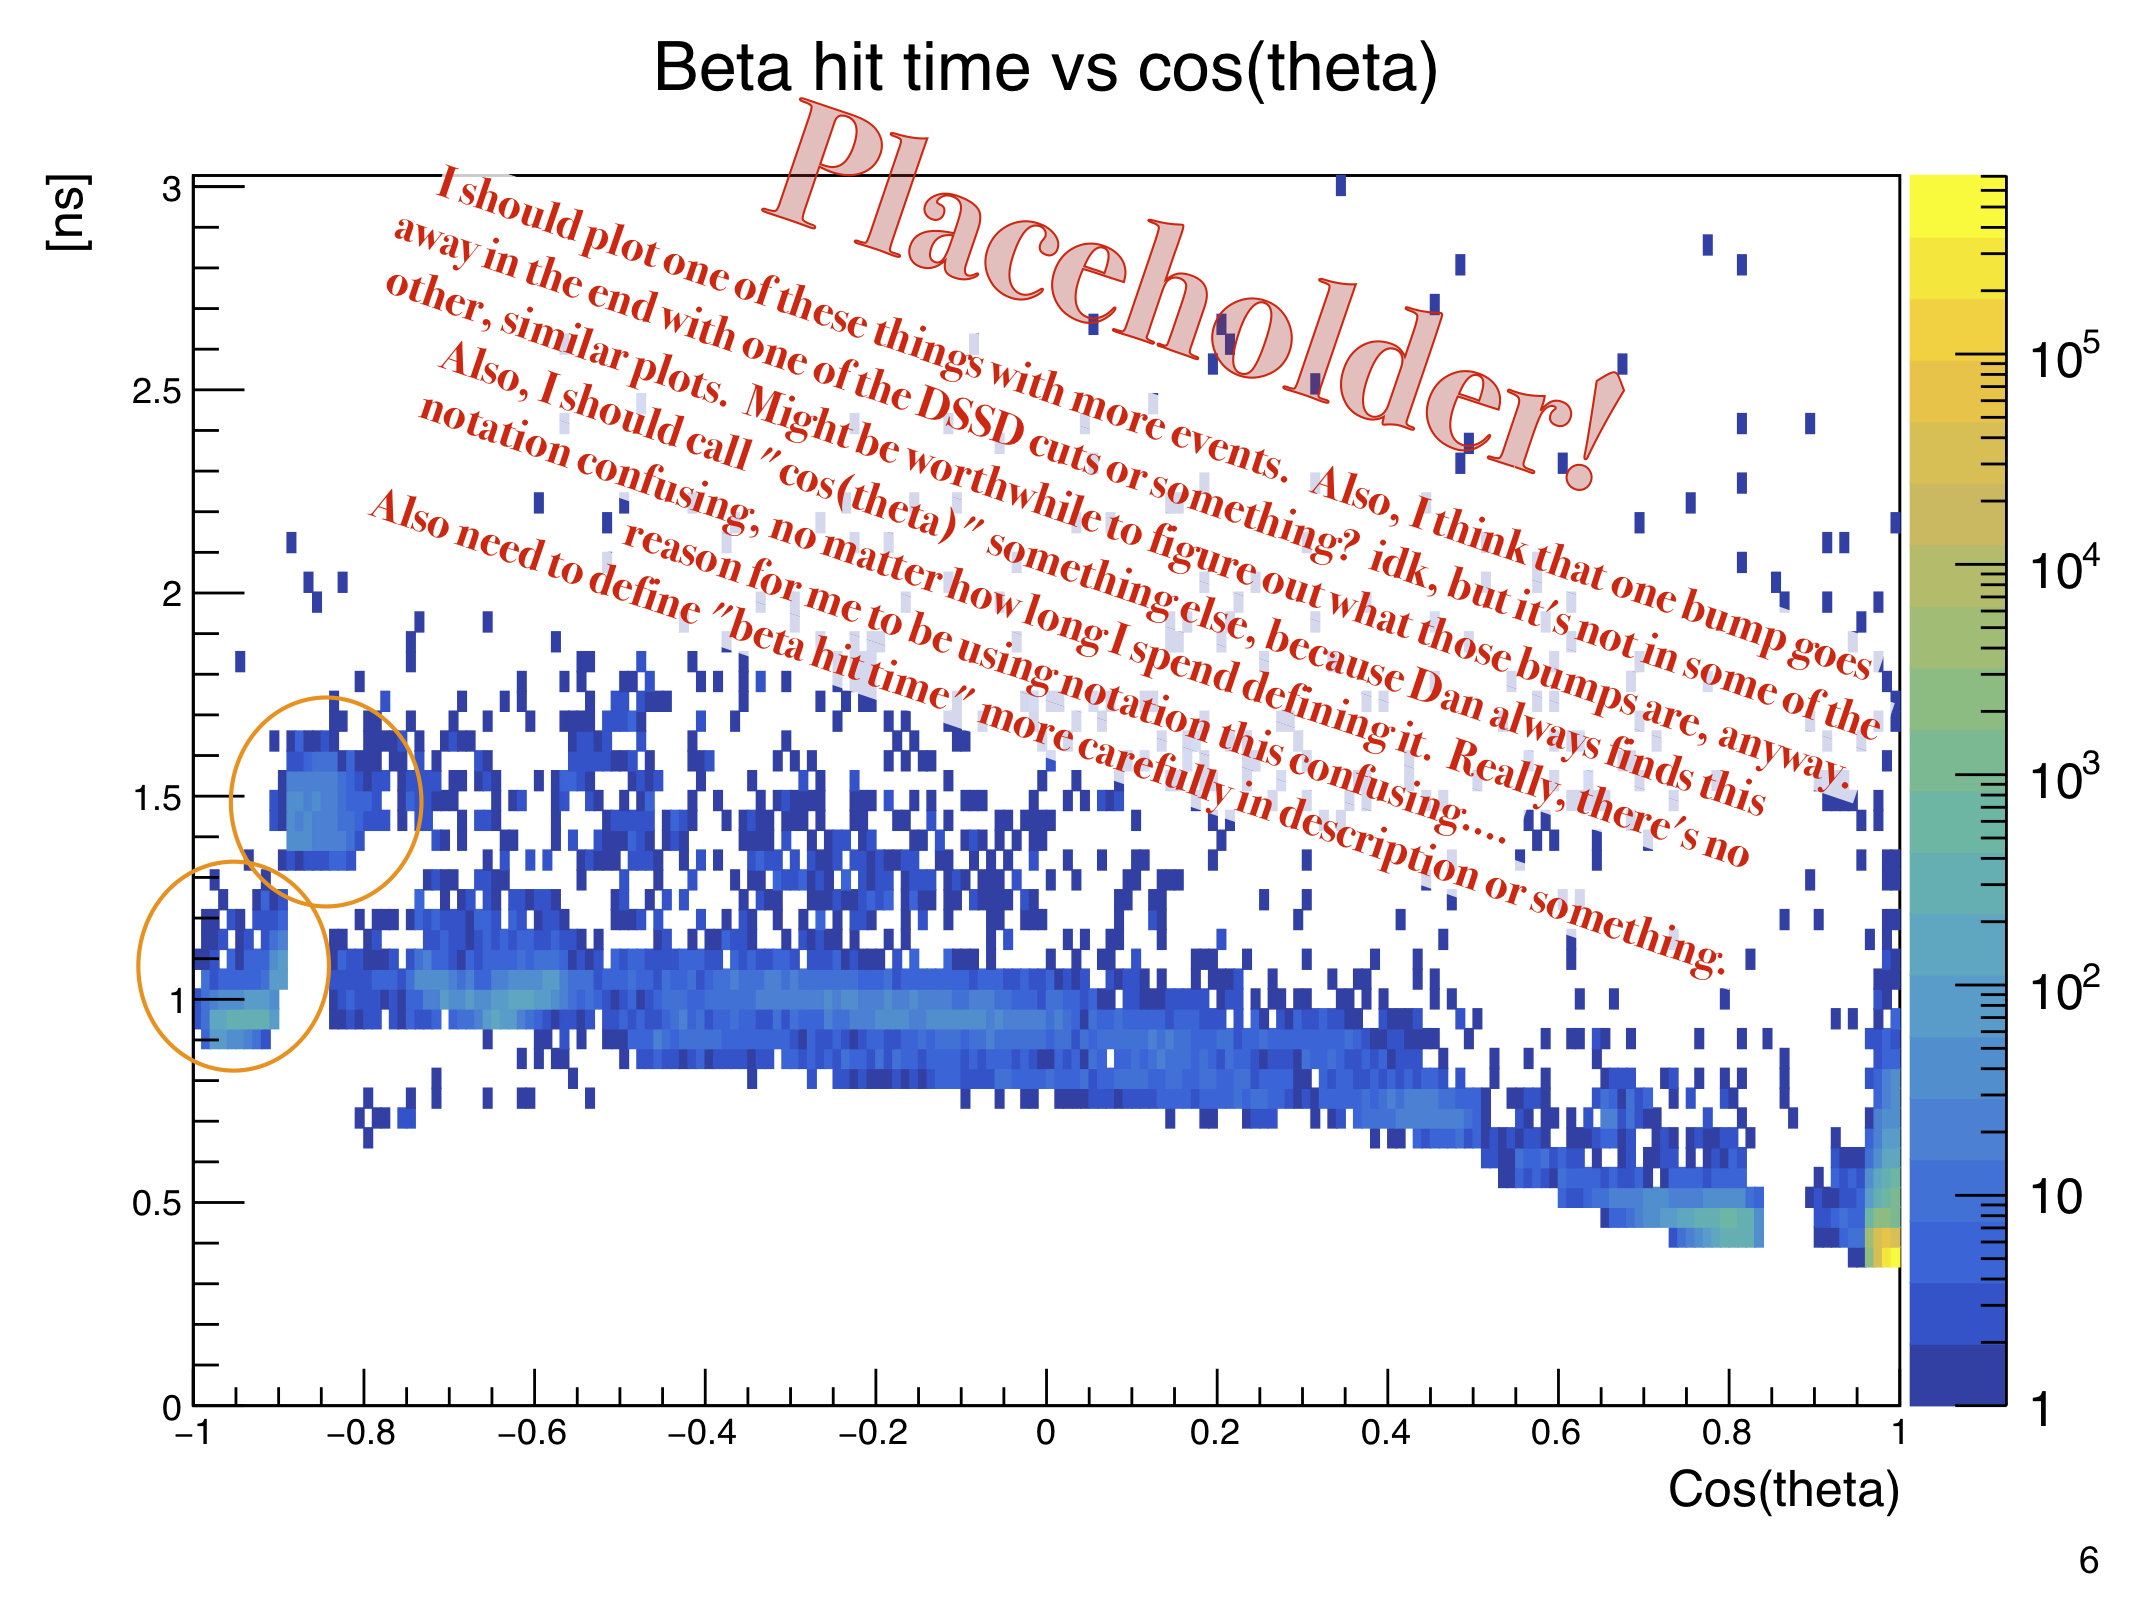
\includegraphics[width=.999\linewidth]
	{Figures/toa_vs_costheta.png}
	\note{This is probably just for the one polarization?  idk.  also, it might be for both detectors, but summed in a non-stupid way.  I have to fix this goddamn picture.}
	\caption[Simulated Beta TOA vs emission angle w.r.t. detector orientation]{Simulated Beta TOA vs emission angle w.r.t. detector orientation.  For betas that eventually hit the top detector, this plot shows the relative angle at which they were originally emitted on the horizontal axis, and on the vertical axis, the travel time from generation to arrival at the detector.  The majority of events observed in the top detector are emitted with initial momentum directed towards this detector.  For events initially directed elsewhere but scattered in, the times of flight grow longer for larger angular deviations.  These events cannot be entirely eliminated in a TOF cut.}	
	\label{fig:toa_vs_costheta}
\end{figure}

%
In order to produce something which can be directly compared with experimental data, a TOF spectrum for SOEs must also be produced and merged with the beta TOF spectrum.  Experimentally, this is done as an event-by-event subtraction, so that is also what must be done for the simulations.  Unfortunately, these two time-of-flight spectra cannot easily be produced within a single type of simulation.  Because scattering is an important effect within the beta time of flight spectra (and resulting beta energy spectra), Geant4 is the tool of choice for this type of particle.  For shake-off electrons, which are emitted with little energy and accelerated through the electric field within the chamber, it is much more important to have an accurate model of the electric field and its effects on charged particles.  The shake-off electrons' time of flight is evaluated by the TRINAT collaboration using COMSOL to track individual electrons through a model of the electric field within the experimental chamber.  
% (created by a series of electrodes held at a constant voltage) 
% , which is generated by a series of electrodes held at a constant voltage.  

The SOEs are treated as being emitted isotropically, with their points of origin distributed according to the density of the central atom cloud.  Three separate TOF spectra are generated, with each corresponding to a different initial distribution of kinetic energy.  The origin of these SOE energy distributions is discussed in Section~\ref{section:soe_intro}.  A final SOE TOF spectrum (relative to the time of decay) was produced by as a linear combination of these three spectra, comprised of $9\%$ 0\,eV events, $77\%$ $4S$ events, and $14\%$ $3P$ events.
%\note{We do the COMSOL thing here too, but it becomes much more useful for the background events, because that's where the electric field is really non-uniform.}
%\note[color=bluetodo]{In the end, we used $(0.09)*(\textrm{0eV}) + (0.91)*(0.85*(\textrm{4S}) + 0.15*(\textrm{3P}))$.   That's $9+77+14$.  I will (eventually) say that *here*, not in the intro section.  Also, John used Eq.20 for the 4S, and Eq.24 for the 3P.}

\begin{itemize}
	\item Combine the SOE TOF spectrum from COMSOL with the beta TOF spectrum from G4.  
	\item Check if it matches the shape of the main peak. --> It does!  Yay.  
	\item In terms of agreement with the experimental spectra, the exact ratio of 4S to 3P doesn't matter much, however adding in the 0eV events makes a big difference.   
	\item Umm.  Did I do a fit for the ratio of 0eV events?  I kind-of don't think I did... 
	\item Also, the SOE events were generated only up to 100 eV.  That smaller number of eV (20??) wasn't enough, even though the tail gets tiny.  Also, for higher energy SOEs, we observe a smaller fraction of the ones that are generated anyway.  
	\note[color=bluetodo]{Umm.  Did I blur the whole peak with statistics?  I don't fucking remember.  I must have.  Check.}
%	\item Umm.  Did I blur the whole peak with statistics?  I don't fucking remember.  I must have.
	\item Also, the SOEs in COMSOL had their original positions picked out by the event generator in G4.  So all the SOEs and betas originated at the same point within the cloud.
\end{itemize}

%%%%%%%%
\note{The collaboration has found that Levinger's formulae fit our measurements of SOE hit position and time-of-flight, in that the distributions are maximal at low energy somewhere, but extend out to higher energies with greatly diminished probabilities.  For our measurement, it turns out to be very important that these distributions not be truncated at too low an energy, however it is much less important which orbital shell the SOEs originated from.  In the case where no electrons are shaken off, we use the model that these electrons are removed instantly from the $^{37}\textrm{\!Ar}$ daughter with no kinetic energy within the lab frame.  Or possibly within their own rest frame.  But we used the lab frame.
\\...\\
Really, this stuff goes in a different chapter somewhere.}

John made some nice plots of these from the eMCP data.  I did *not* use it to make a cut on eMCP hit position in the end, despite the fact that it makes the spectrum more clean, because a lot of good events don't have full hit position information, and you lose an awful lot of statistics by making the cut.  I used this for modeling the background spectrum, but in the end it wasn't as elegant a result as I might have hoped.  Also, it's still an open question exactly which fraction of SOEs come from which atomic shell, but it doesn't change the resulting spectrum very much.

\note[color=jb]{JB on 2.4 SOE:
\\
Say what you did, with as little info as possible now. Georg is a theoretical
chemist, so he may be very curious about this.
\\ ... \\
"Atomic electrons with kinetic energies 0 to 100 eV are produced as part
of the beta decay process.
If their energy is below a certain value, our detection process is not perturbed,
so we provide physics about the energy spectrum here.
\\ ... \\ 
Levinger~\cite{Levinger}, assuming the sudden approximation,
calculated the overlap between an electron in the initial  atom with
an outgoing electron or an electron in  the final atom. Levinger approximated
everything with hydrogenic wavefunctions, so his calculations become
analytic. The collaboration has found that Levinger's formulae
fit our measurements of the position and TOF  info of our atomic electrons,
so they are used in our simulations 
\\
OR
\\
but the precise energy spectrum was found to be unimportant, so we used X in our
simulations.
\\
whichever is true.
\\...\\
This is then fine. You have most of the basics down.
}




%	\missingfigure{Show simulated $\cos\theta$ vs TOF.  You can just make a lot of that go away with a properly selected cut.}

%\note[color=jb]{JB says:  
%Please discuss this at the next meeting.  (ETA:  Done!)
%\\
%Indeed this is why you should avoid calling the events originating not from the trap 'scattered events.' More importantly, why it was so critical that you reduced the size of the correction by timing bad events out. I would say you have a well-determined TOF cut to minimize this error-- a cut that could not have been done blind without an unreasonably perfect simulation.  Thus the exact spot of the cut should not be considered to introduce a systematic. }




%%%%%%%%%%%%%%%%%%
\section{Simulating the Background and Time of Flight}
%\section{Scattering and Background within the SOE TOF}
\label{sec:tof_bg}
One of the largest sources of background events in this experiment is from decaying $\isotope[37]{K}$ atoms that have escaped from the trap and become stuck on the other surfaces within the chamber.  The majority of these events can be eliminated simply by taking a time-of-flight cut on the eMCP relative to a scintillator hit time (as described in Section ~\ref{section:emcp_cuts}).  Unfortunately, this procedure cannot remove the entirety of the background, so what remains--both background events from chamber surfaces, and events from the atom cloud itself--must be modeled and understood.  

The model used for events originating from the atom cloud is described in Section~\ref{sec:bs}, and this section will discuss events originating from other surfaces within the chamber.  The methodology used is very similar.  

%%%%%%%%
To this end, spectra for both the beta time of flight and shake-off electron time of flight (calculated with respect to the time of decay) are generated, both for events originating from the cloud and for events originating from surfaces within the chamber.  The beta TOF and SOE TOF spectra are combined by an event-by-event `subtraction', producing the simulated equivalent of an ``experimental SOE TOF'' spectrum (which, of course, is only a \emph{true} time-of-flight spectrum in the limit where the beta travel time is zero -- that is, since we cannot know the true time of decay, 

%not a true time-of-flight spectrum, since it simply subtracts the beta hit time from the SOE hit time).  
%experimental spectra that we might otherwise have described as a ``SOE TOF'' spe
% from one another event-by-event to produce a spectrum to mimic the experimental ``SOE TOF'' spectrum (SOE hit time minus beta hit time).  

The two spectra are generated separately because different software is required for each type of particle.  The lower energy shake-off electrons may have their paths perturbed by any non-uniformities within the ambient electric field.  This is of particular concern in the regions far from the central path between the atom cloud and the eMCP, where non-uniformities are at their largest -- the very same regions from which many of these background events originate.  This is not the regime in which Geant4 is designed to operate. Furthermore, it turns out to be non-trivial to adequately model a non-uniform electric field within this framework.  As a result, the shake-off electron spectra were generated by the collaboration using COMSOL to model precise shape of the electric field within our experimental geometry.  

%\note{initial SOE spectra were something something levinger.} 

The beta time of flight spectra from surfaces within the experimental chamber were generated with Geant4, in order to account for variations in travel time arising from beta scattering.  This also allows us to simultaneously account for energy lost to scattering within this background spectrum.

%...the beta TOF spectrum must be generated through Geant4 in order to account for the different time of flight for betas that...

%Though the betas are relativistic, it is insufficient
%While the betas are relativistic, it is insufficient to 

%Although these betas are relativistic, it is insufficient to calculate their TOF by simply taking the path length and dividi



We model the beta TOF from the surfaces in G4, event by event.  This is necessary because scattered \aside[color=jb]{JB:  ``I wouldn't call these "scattered" events... that's very misleading.'' 
	\\ ... \\ 
	Yeah, I should really stop doing that.  
	\\ ... \\ 
	Wait no, scattered is what I mean!  But fine, my phrasing is really unclear.} events will have their TOF changed to account for a longer beta pathlength, and we're preferrentially cutting away the events that don't have a TOF in the appropriate range.  ....And then have COMSOL generate electron TOFs for SOEs starting from the start points picked by G4.  Ran COMSOL for 0 eV SOEs, and again for Levinger spectrum SOEs.  Used ~9\% 0eV SOEs in the end.  I forget which Levinger distribution I used in the end.  \aside[color=jb]{JB:  Please comment on whether or not it was important to have this energy distribution.}  The point is, for each event, you've simulated a beta TOF that may or may not be scattered off of something before it hits a detector, and you have a SOE TOF for an event originating at that same point, so you subtract them to model the TOF you'd measure in an experiment.  Also, because you've done the scattering with G4, you get the beta energy corrected for any scattering that happened.  This way, one can estimate %\aside[color=jb]{JB:  `you know precisely' $\rightarrow$ `you can estimate'} 
how many ``bad" events are eliminated with the TOF cut, as well as the fraction of ``bad'' events left in what remains.


\begin{figure}[h!tb]
	\centering
	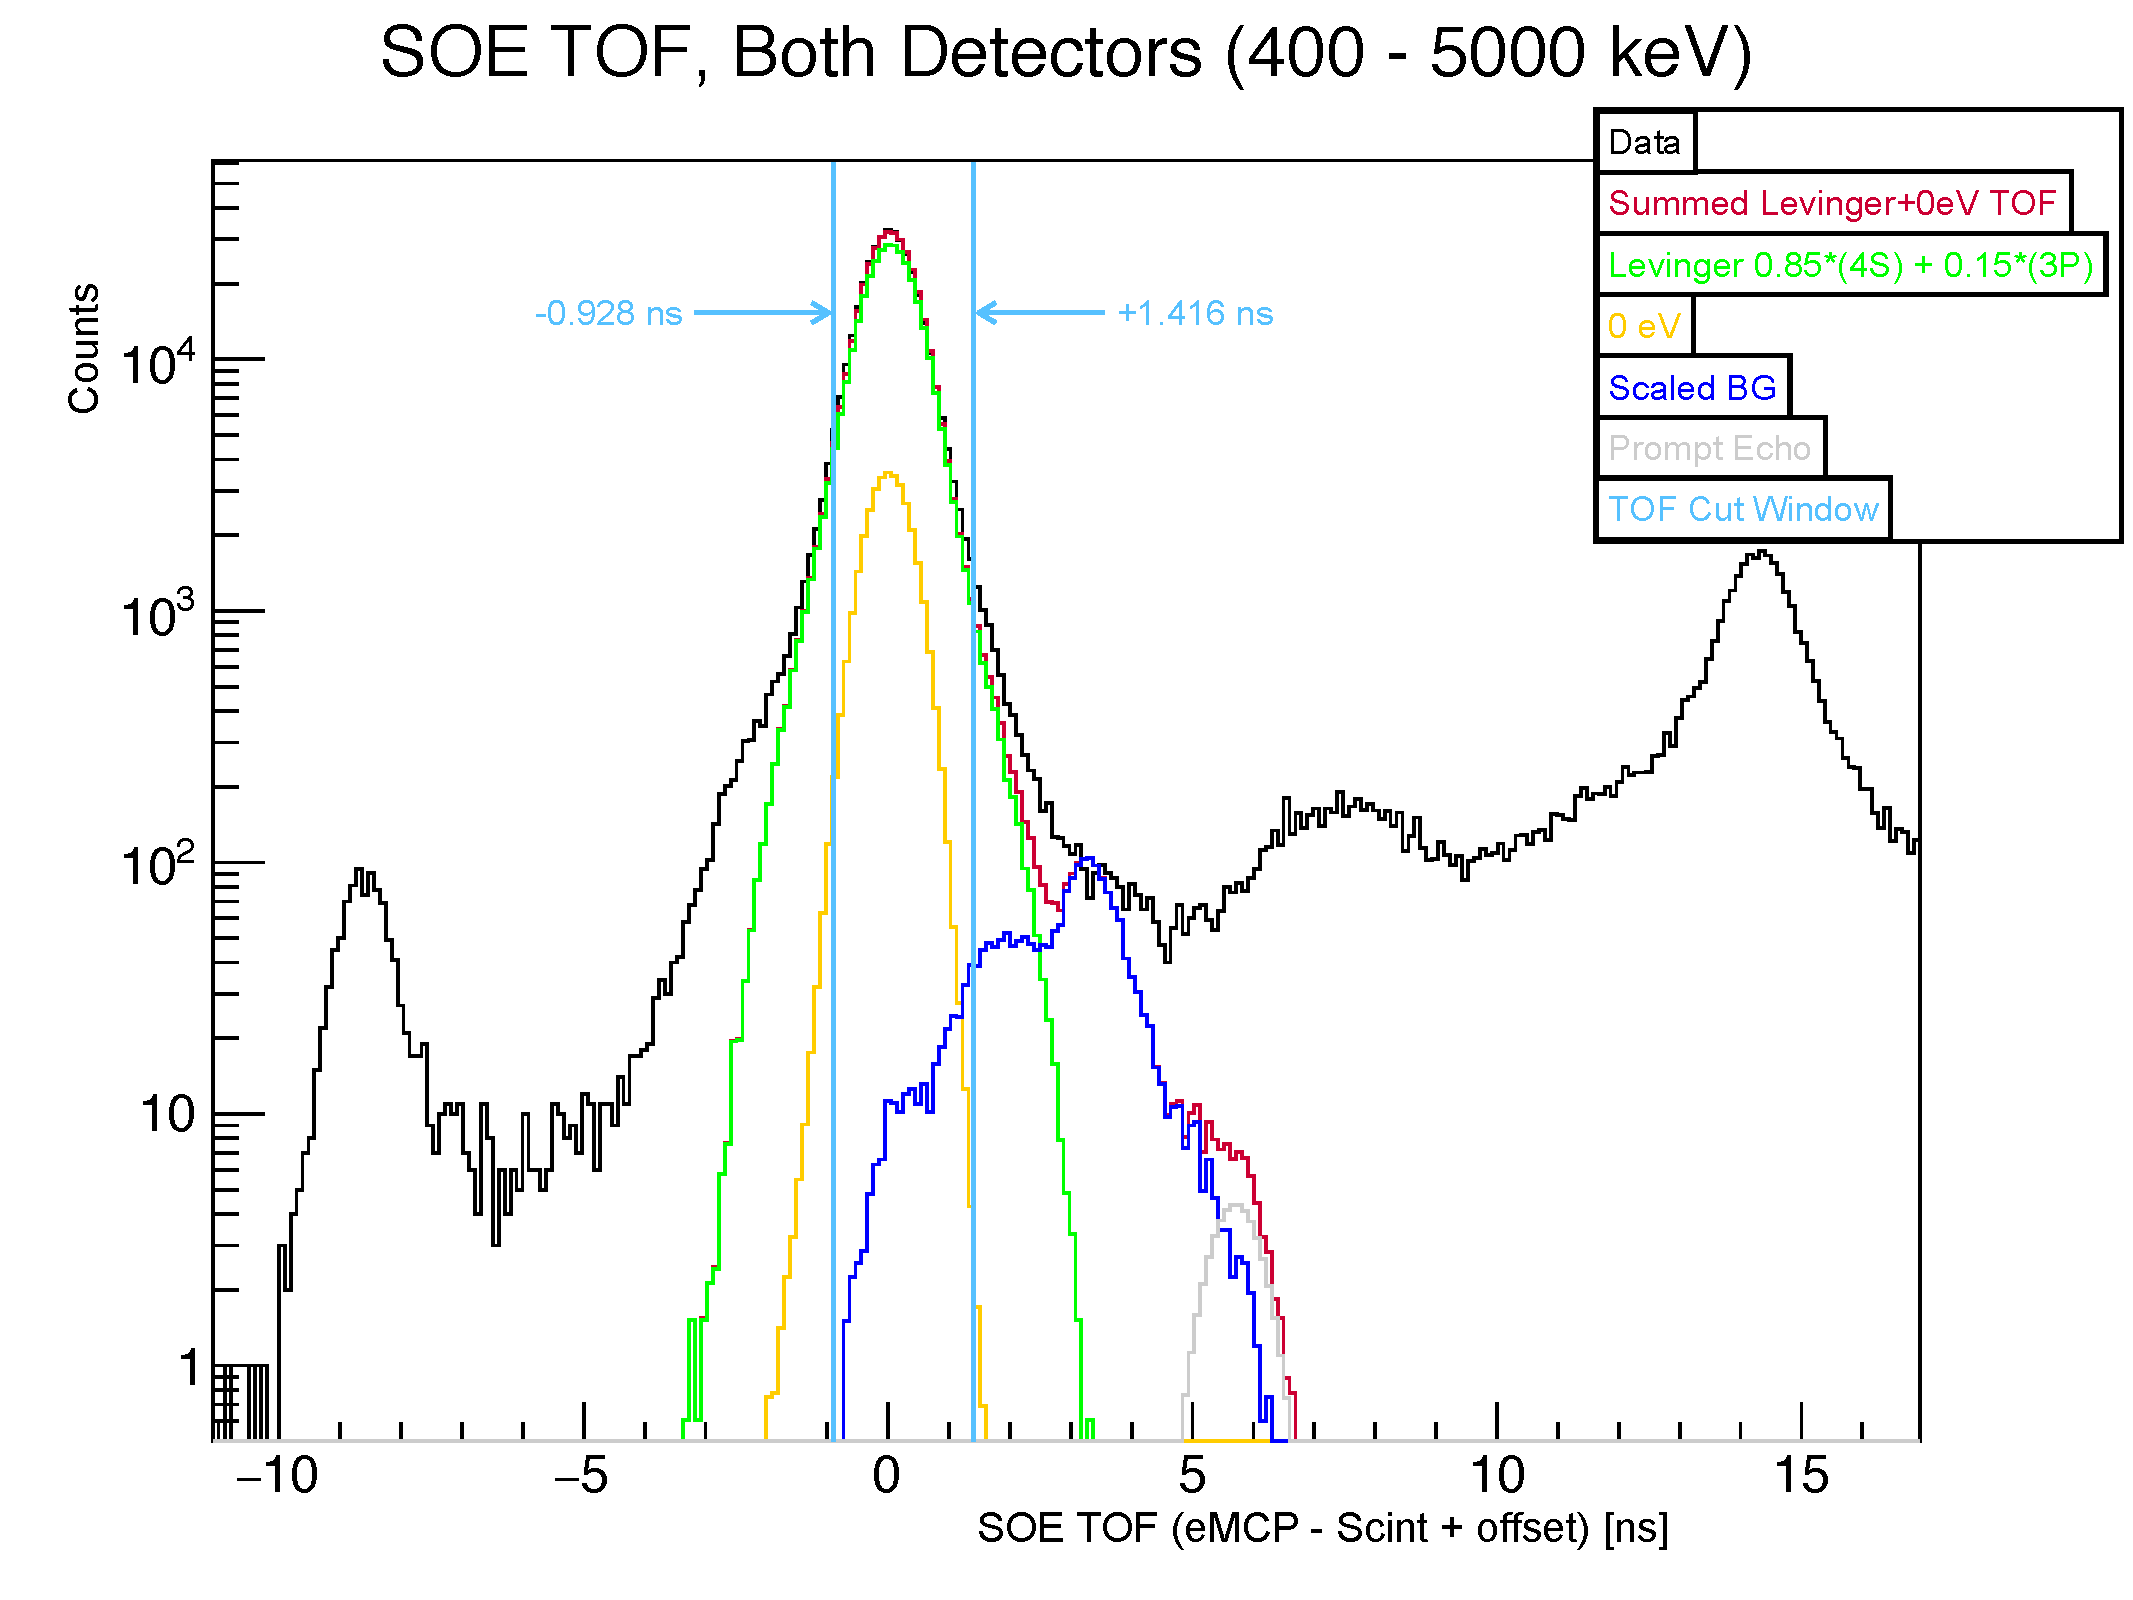
\includegraphics[width=.999\linewidth]
	{Figures/SOE_TOF_Spectra.pdf}
	\note{Rephrase.}
	\note{Reference Section~\ref{section:emcp_cuts}, probably.}
	\caption[SOE TOF -- Model and Data]{SOE TOF, with both model and data.  In the end, the data was cut to use only events with a TOF between -0.928 ns and +1.416 ns.  Max. possible background is like a factor of two too big.  Similar quality results no matter how you distribute the Levinger spectra between 4S and 3P, however adding the 0 eV electrons makes a big improvement to the agreement. }	
	\label{fig:soetof}
\end{figure}

%Our experiment has some background.  It's annoying and stupid, but as long as we can estimate how much of it there is and what it does, it's basically fine.

\begin{itemize}
		\item TOF cut requires a whole extra model of background in the TOF spectrum..
		\item Suppose background in the TOF spectrum is coming from decays of atoms that have gotten themselves stuck to surfaces within the chamber...
		\item Run G4 to get a beta TOF spectrum (w.r.t. the decay)
		\item Run COMSOL (credit to Alexandre) to track low-energy SOEs through the electric field from wherever they started, into the detectors.  Energy spectra from Levinger.
		\item Combine G4 and COMSOL spectra, event-by-event, while requiring that both the beta detector and the eMCP are hit according to the set of random numbers generated by each monte carlo separately.  Then, the beta and SOE will each have a TOF from decay to detector, and subtracting one from the other gives a timing spectrum that can be observed experimentally.  See Fig.~\ref{fig:soetof}.
		\item Upper limit for the fraction of events generated this way can be estimated by assuming that all losses from the trap not due to radioactive decay emerge isotropically from the trap and then stick to whatever chamber wall is in its path.  This upper limit is too big by a factor of 2.
	\item For each of those 3 simulations, sort the ``good'' data according to emission angle relative to the detector.  Do each detector individually.  For both polarizations.
	\item Assemble the (simulated) superratio asymmetry.  We'll compare it to data, and the $\chi^2$ from that comparison will be our figure of merit.  
	\item We can make a whole 2D parameter space for different values of $\Abeta$ and $\bFierz$, and compare them all (via their superratio asymmetries) to the experimental data.  We get the ``best'' values of $\Abeta$ and $\bFierz$, where $\chi^2$ is minimized.
	\item We can do this whole thing again for simulated data sets with different values of parameters that we vary as systematics.  Note how the best values of $\Abeta$ and $\bFierz$ change when each of the systematics are varied.
\end{itemize}

\begin{figure}[h!tb]
	\centering
	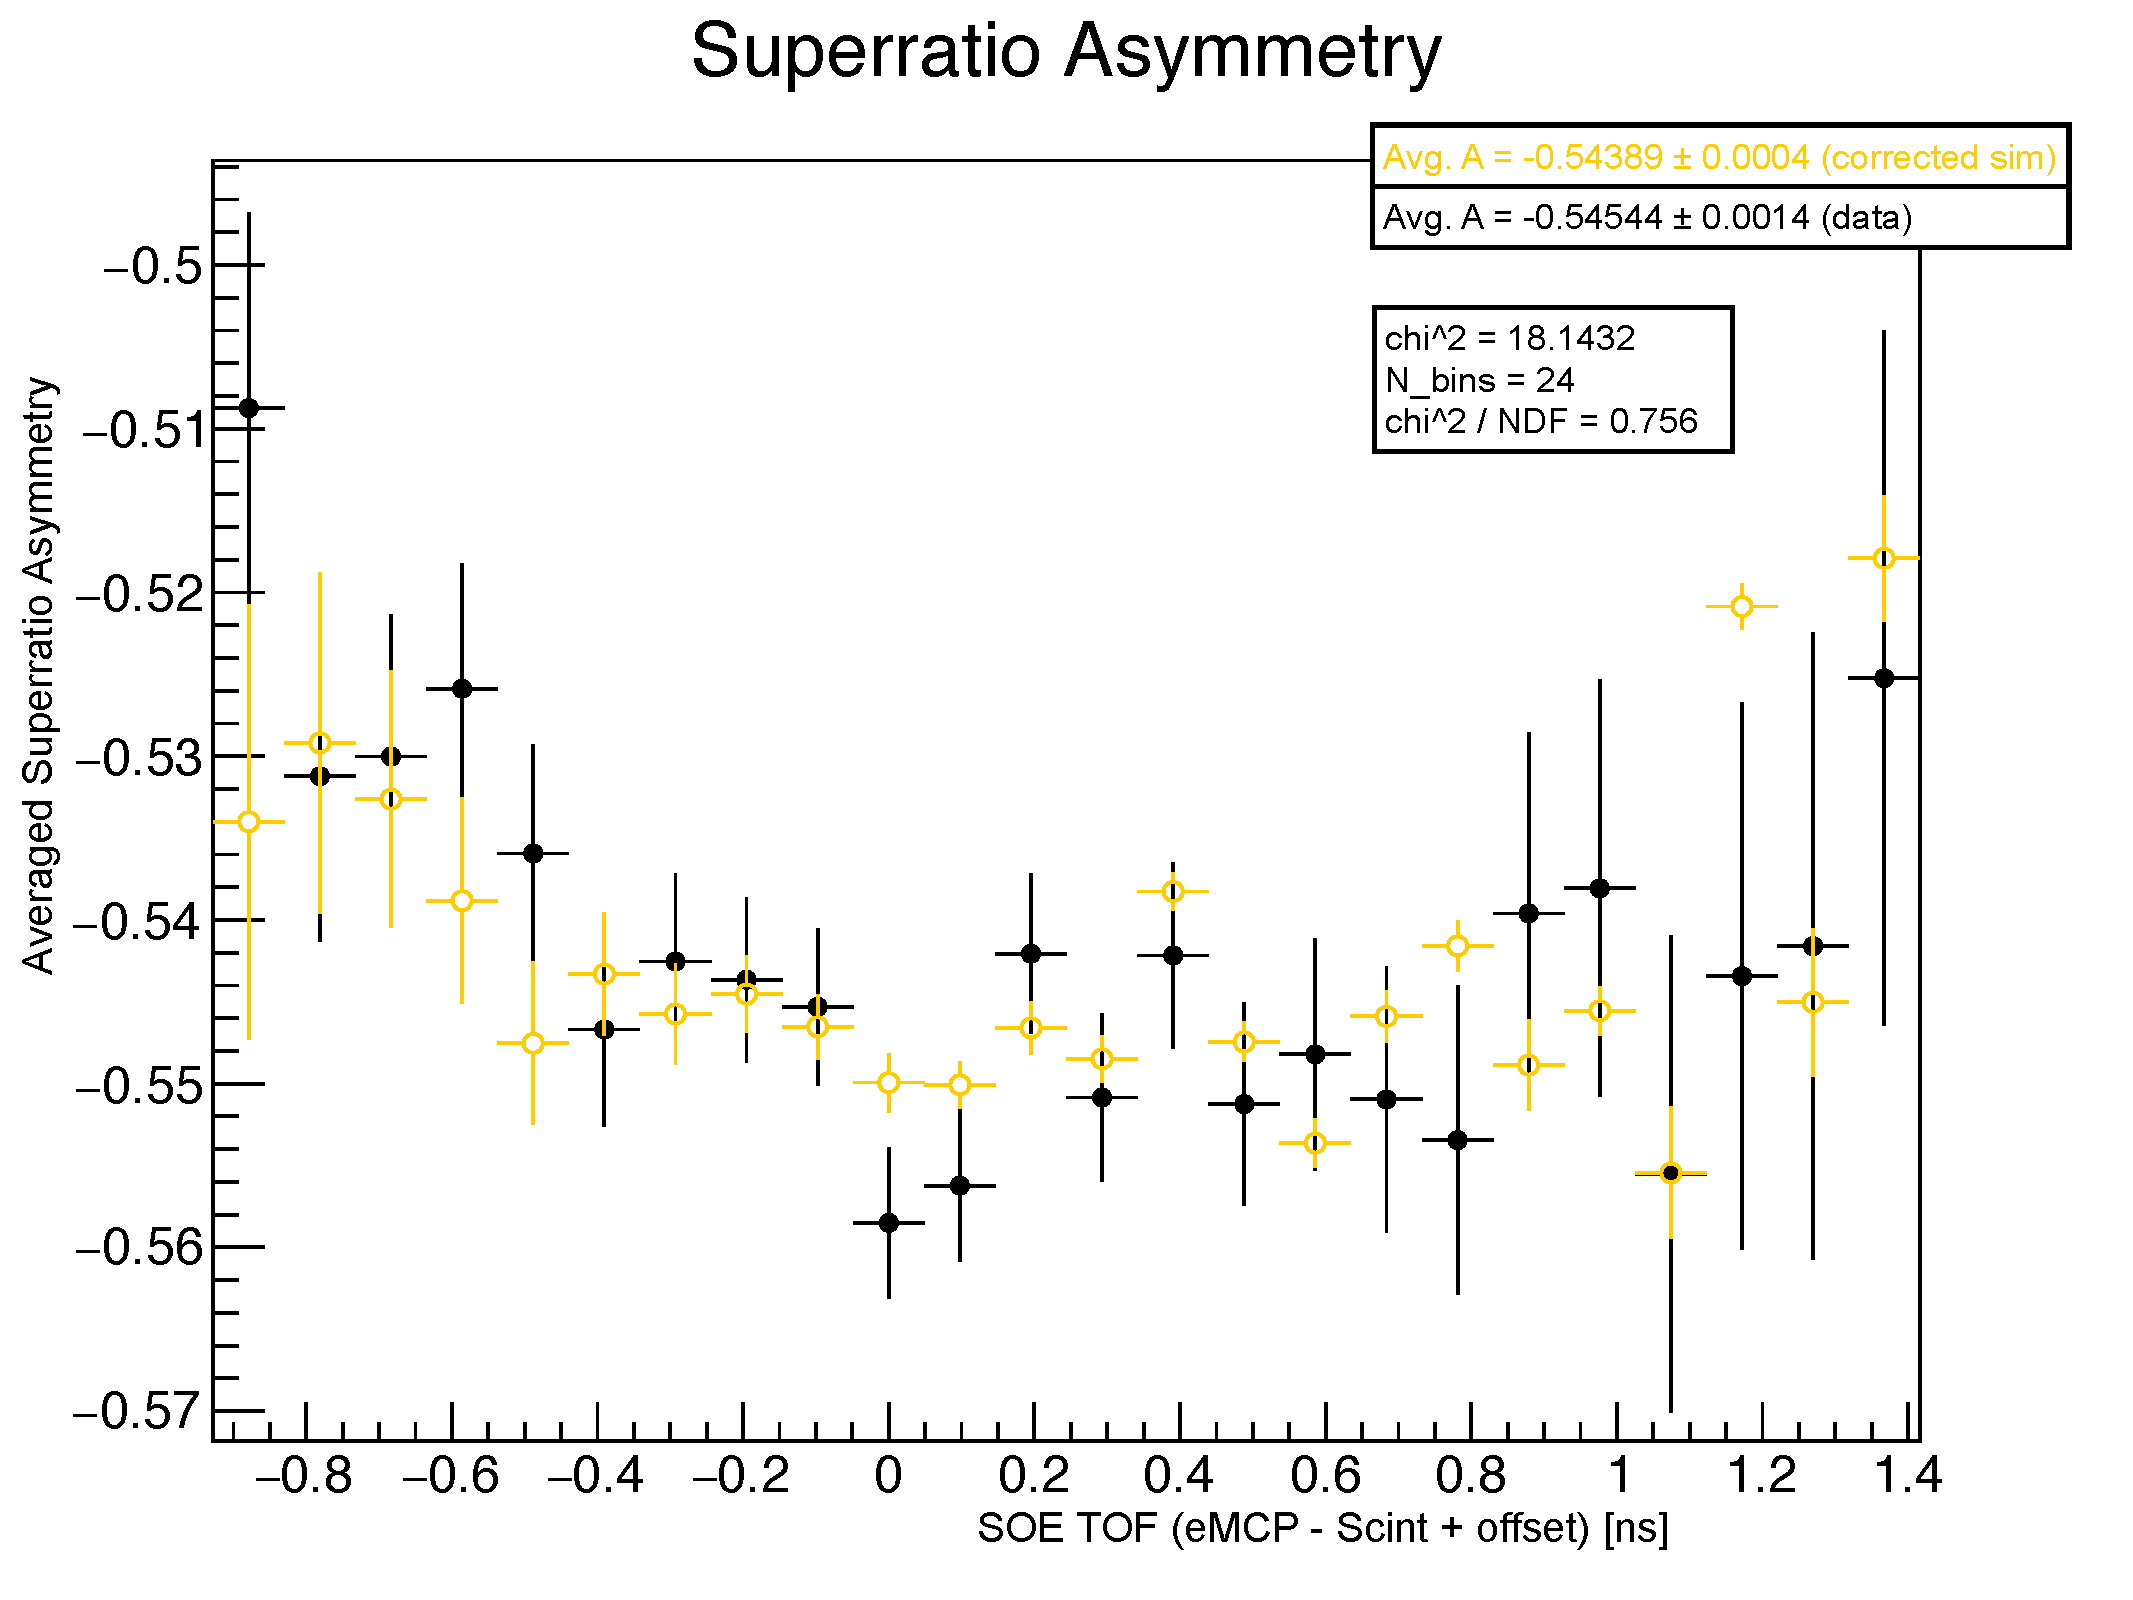
\includegraphics[width=.999\linewidth]
	{Figures/asymmetry_by_tof.pdf}
%	\note{I think I want this picture to go in some other section.}
	\note{Show the "average asymmetry" (all energies) as a function of TOF, with real data, best model normalization, and extrema of model normalizations.  Show our cut.  Turns out, it's a lot of work for a really tiny correction.  Oh well.}
	\note[color=jb]{JB on the *actual* figure I had been planning to put here, and my remarks about it:  Indeed it will be critical to show a clear compelling version of this figure in thesis and in a paper.  It was vital to minimize and determine this background to avoid fitting a polynomial to it from the wings,  even more so for the energy dependence of A than for its average -- you should say so.
	\\ ... \\
The reason the correction is small is because of all your hard work.}
	\caption{The superratio asymmetry, averaged over all scintillator energies between 400-4800 keV, is used to compare the experimental data and simulated TOF model as a proxy for the quality of the model to estimate the background.  All other cuts have been applied.}	
	\label{fig:asymmetry_by_tof}
\end{figure}


%\subsection{Begin Imported Section!  ``Background Modeling -- Decay from Surfaces within the Chamber''}
%	So many surfaces, all of which can get stray 37K atoms stuck to them.  Then they decay from a place that isn't the actual trap center, and it contaminates our stuff.
%	\missingfigure{Show modelled TOF spectra in comparison with real TOF spectra.  Show the cut we made on that. }
%	\note[color=jb]{JB on figures that might go here:  Figure 6.4 (currently that picture of the TOF spectrum) could either be here, or you could reference it from here. The TOF histogram is a great start. Adding the asymmetry[TOF] indeed would be vital.}


%	\subsection{Decay from Chamber Surfaces}



%%%%\clearpage
%%%%\FloatBarrier
%%%\section{OldSection -- ``Comparing Simulations to Experimental Data''}
%%%\note[color=org]{This content got moved to Ch.~\ref{sec:comparing_data_sims}.}
